%\documentclass[3p,12pt,authoryear]{elsarticle}
\documentclass[3p,12pt]{elsarticle}
\let\counterwithout\relax
\let\counterwithin\relax
\usepackage{natbib}
\usepackage[colorlinks=true,citecolor=blue,linkcolor=blue]{hyperref}
\usepackage{amsmath,amssymb}
\usepackage{epsfig}  
\usepackage{graphicx}               % Standard graphics package  
\usepackage{url}
\usepackage{titlesec}
\usepackage{hyperref}
\usepackage{cleveref}
\usepackage{color}
\usepackage{listings}

\usepackage{titlesec}

\setcounter{tocdepth}{4}
\setcounter{secnumdepth}{4}

\usepackage{tikz}
\usetikzlibrary{trees}

\tikzstyle{every node}=[draw=black,thick,anchor=west]
\tikzstyle{selected}=[dashed,draw=red,fill=red!30]
\tikzstyle{optional}=[dashed,fill=gray!50]

\usepackage{chngcntr}
\counterwithin{figure}{section}

\titleclass{\subsubsubsection}{straight}[\subsection]
\newcounter{subsubsubsection}[subsubsection]
\renewcommand\thesubsubsubsection{\thesubsubsection.\arabic{subsubsubsection}}
\renewcommand\theparagraph{\thesubsubsubsection.\arabic{paragraph}} % optional; useful if paragraphs are to be numbered

\titleformat{\subsubsubsection}
  {\normalfont\normalsize\itshape}{\thesubsubsubsection}{1em}{}
\titlespacing*{\subsubsubsection}
{0pt}{3.25ex plus 1ex minus .2ex}{1.5ex plus .2ex}

\newcommand{\bra}[1]{\ensuremath{\left\langle#1\right|}}
\newcommand{\ket}[1]{\ensuremath{\left|#1\right\rangle}}
\newcommand{\bracket}[2]{\ensuremath{\left\langle#1 \vphantom{#2}\right| \left. #2 \vphantom{#1}\right\rangle}}
\newcommand{\matrixel}[3]{\ensuremath{\left\langle #1 \vphantom{#2#3} \right| #2 \left| #3 \vphantom{#1#2} \right\rangle}}
\newcommand{\bls}{\begin{lstlisting}}
\newcommand{\els}{\end{lstlisting}}

\newcommand{\ttf}{\ttfamily}

\newcommand{\pa}[2]{\frac{\partial #1}{\partial #2}}
\newcommand{\p}[1]{\partial_{#1}}

\definecolor{mauve}{rgb}{1,0,1}
\definecolor{dkgreen}{rgb}{0,0.6,0}
% \definecolor{gray}{rgb}{0.5,0.5,0.5}
% \definecolor{mauve}{rgb}{0.58,0,0.82}

\lstset{language=C++,
%   aboveskip=3mm,
%   belowskip=3mm,
%   showstringspaces=false,
%   columns=flexible,
   basicstyle={\small\ttfamily},
%   numbers=none,
%   numberstyle=\tiny\color{gray},
   morekeywords={SU\_vector,string,Body,Track,marray,Basis},   
   keywordstyle=\color{blue},
   deletekeywords={const},
   keywords=[2]{const},
   keywordstyle={[2]\ttfamily\color{red}},
   deletekeywords={operator},
   keywords=[3]{operator},
   keywordstyle={[3]\ttfamily\color{dkgreen}},
   commentstyle=\color{dkgreen},
   stringstyle=\color{mauve},
%   breaklines=true,
%   breakatwhitespace=true
%   tabsize=3
}

\setcounter{secnumdepth}{4}
\setcounter{tocdepth}{4}

\begin{document}

\begin{frontmatter}

\title{$\nu$-SQuIDS: A toolbox for neutrino oscillations\tnoteref{t1}}

\author[MIT]{Carlos A. Arg\"uelles}
\ead{caad@mit.edu}
\author[UB]{Jordi Salvado}
\ead{jsalvado@icc.ub.edu}
\author[UA]{Christopher N. Weaver}
\ead{chris.weaver@icecube.wisc.edu}
\address[MIT]{Massachusetts Institute of Technology, Cambridge, MA 02139, USA}
\address[UA]{Dept.~of Physics, University of Alberta, Edmonton,
  Alberta, Canada T6G 2E1} 
\address[UB]{Departament de F\'isica Qu\`antica i Astrofísica and Institut de Ciencies del Cosmos,
Universitat de Barcelona, Diagonal 647, E-08028 Barcelona, Spain}

\tnotetext[t1]{The code can be found in \url{https://github.com/arguelles/nuSQuIDS}}
\journal{arXiv}
%\journal{Computer Physics Communications}

\begin{abstract}
The Neutrino Simple Quantum Integro-Differential Solver ($\nu$-SQuIDS)
is a C++ code based on SQuIDS that propagates an ensemble of neutrinos
through a given media. Neutrino oscillation calculations relevant to
current and next generation experiments are implemented. In doing so
we account for coherent and non-coherent neutrino interactions in
different media such as the Sun, Earth, Vacuum, or others.
The code has been design to be accurate and flexible, while at the
same time maintain good performance. It has a modular design that
allows the user to incorporate new physics in novel scenarios. 
\end{abstract}

\begin{keyword}
Neutrino oscillation, phenomenology, collective neutrino behavior, numerical techniques
\end{keyword}

\end{frontmatter}

\hypersetup{linkcolor=black}
\tableofcontents
\hypersetup{linkcolor=blue}
\newpage
\section{Introduction}
\label{sec:intro} 

In recent decades a plethora of evidence that neutrinos change
flavor as they propagate macroscopic distances due to the
non-alignment of their mass and flavor eigenstates~\citep{Mohapatra:qv, Gouvea:2013fj} has accumulated from
solar~\citep{Abe:2010hy, Borexino2014},
atmospheric~\citep{PhysRevD.91.072004,Richard:2015aua},
accelerator~\citep{PhysRevLett.112.181801,
  PhysRevD.93.051104,PhysRevLett.116.151806, PhysRevLett.110.251801}, and
reactor \citep{An:2013zwz,Abe:2015rcp, Kim:2016yvm} experiments.
Thanks to these remarkable
experimental results and related theoretical calculations the
  neutrino-mass induced flavor oscillation paradigm
\citep{Pontecorvo:1967fh,Gribov:1968kq,fukugita2003physics,
  Akhmedov:1999uz,Balantekin:2013kc, GonzalezGarcia:2007ib}
has been firmly established and the three mixing angles, which
parametrize the lepton mixing matrix, together with the two squared
mass differences, have been measured to good precision
\citep{Gonzalez-Garcia:2014bfa}. It is the task of on-going 
and future experiments to determine the neutrino mass ordering
and the Dirac CP-violating phase \citep{Hewett:2012et,
  Acciarri:2016crz,Aartsen:2014oha, Kouchner:2016pqa,DeRosa:2016ifc}. 
Also, the IceCube Neutrino Observatory has recently made precise measurements of the atmospheric
spectrum above 100 GeV allowing new physics
models to be constrained \citep{Aartsen:2014gkd,TheIceCube:2016oqi}.
The identification of high energy
extraterrestrial neutrinos \citep{ Aartsen:2014gkd, Aartsen:2015rwa}
has opened the possibility of exploring new physics at these energies as well
\citep{Arguelles:2015dca, Bustamante:2015waa, Baerwald:2012kc}. 

Matter effects play a fundamental role in the explanation of solar
neutrinos \citep{ Davis:1968cp,Bethe:1986ej}, which has motivated the study of new flavor
changing neutrino interactions \citep{Barger:1991ae, Roulet:1991sm, GonzalezGarcia:2011my,
  Gonzalez-Garcia:2013usa, Pospelov:2011dp, Kopp:2014nosterile,
  Maltoni:2015kca}.
Even though most of the data can be explained in the standard three
neutrino framework, some puzzling anomalies still remain
\citep{LSND,Mention:2011rr,MiniBoone:2012dn}. These may be explained
by introducing new light neutrino states \citep{kopp2013sterile,
  Collin:2016rao, Abazajian:2012rf} and other new physics
\citep{Bai:2015ztj,PalomaresRuiz:2005vf,Gninenko:2011xa}.
Also, the interplay between cosmology and neutrino
oscillation has been widely studied in the literature
\citep{Bergstrom:2014fqa, Giusarma:2016phn,
  Dasgupta:2013la,Hernandez:2016kel,Arguelles:2016uwb}. 
% the following sentence doesn't really make sense:
In general, neutrino physics constitutes an excellent proof for
fundamental physics \citep{Hewett:2012et}.

Tools are needed to accurately and reliably compute neutrino
oscillation phenomenology, i.e. vacuum oscillation and matter
interactions. In particular, when only neutrino
oscillations are important libraries such as {\ttf GLoBES}
\citep{Huber:2007ji}, {\ttf Prob3++} \citep{prob3pp, Calland:2013vaa},  and {\ttf
  nuCRAFT} \citep{Wallraff:2014vl} are available. Unfortunately, when non-coherent interactions are
important they are no longer applicable. Furthermore, the ability to
allow the user to incorporate new physics models or to change the
propagation medium is also limited. {\ttf nuSQuIDS} seeks to
address all of these problems by providing a highly customizable
package, while at the same time remaining numerically efficient.

The rest of the paper is organized as follows: in section \ref{sec:theory} we review neutrino oscillation theory and establish notation; in section \ref{sec:code} we describe the code; in section \ref{sec:examples} we demonstrate the use of the code and test it in benchmark scenarios. Finally, section \ref{sec:conclu} presents concluding remarks.

\section{Neutrino Oscillations}
\label{sec:theory} 
In this section we are briefly review neutrino oscillations
using the density matrix formalism.
We can represent the state of the neutrino ensemble, at an energy $E$
and position $x$, using the density
matrix, i.e. in the weak-interaction flavor eigenstate basis
$\{\ket{\nu_\alpha}\}$  it can be written as

\begin{equation}
\rho(E,x) = \sum_\alpha \phi_\alpha(E,x) \ket{\nu_\alpha}\bra{\nu_\alpha} , 
\label{eq:state}
\end{equation}
where $\phi_\alpha$ specifies the flavor content. Another important
basis is the mass eigenstates $\{ \ket{\nu_i}  \}$, which are the
eigenstate of the propagation in vacuum and are related to the former by
\begin{equation}
\ket{\nu_\alpha} = \sum_i U^*_{\alpha i} \ket{\nu_i} ,
\label{eq:changebasis}
\end{equation}
where $U$ is known as the Pontecorvo-Maki-Nakagawa-Sakata (PMNS)
mixing matrix. For antineutrinos the relation is the same as in
\eqref{eq:changebasis} with $U \to U^*$.
It is customary to parametrize the mixing matrix $U$
with mixing angles, $\{\theta_{ij}\}$, and CP phases, $\{ \delta_{ij}
\}$, for example when considering the standard three flavor paradigm
the following parametrization is often used
\begin{equation}
U
=
\begin{pmatrix}
c_{12} c_{13} & s_{12} c_{13} & s_{13} e^{-i\delta_{13}} \\ 
- s_{12} c_{23} - c_{12} s_{23} s_{13} e^{i\delta_{13}} & c_{12} c_{23} - s_{12} s_{23} s_{13} e^{i\delta_{13}} & s_{23} c_{13} \\
s_{12}s_{23} -c_{12}c_{23}s_{13}e^{i\delta_{13}} & - c_{12} s_{23} - s_{12} c_{23} s_{13} e^{i\delta_{13}} & c_{23} c_{13}
\end{pmatrix}
\,,
\label{eq:U}
\end{equation}
where $c_{ij} = \cos \theta_{ij}$, $s_{ij} = \sin \theta_{ij}$. In the
three flavor scenario we use the aforementioned parametrization (with
values from \citep{Gonzalez-Garcia:2014bfa}) and when more flavors are
considered we used the prescription given in
\cite{SQUIDS}. Furthermore, the neutrino ensemble propagation is
described by the following quantum Von Neumann equation \footnote{We set $c = \hbar = 1$.} 
\begin{equation}
\pa{\rho(E,x)}{x} = -i [ H (E,x), \rho(E,x) ].
\label{eq:schrodinger}
\end{equation}

In general we can always split the Hamiltonian, $H$, into a time dependent and independent parts. In particular, for neutrino oscillations the following splitting is convenient
\begin{subequations}
\label{eq:hamiltonian}
\begin{align}
H(E,x) &= H_0(E)  + H_{1}(E,x) ,\\
H_0 (E) &= \frac{1}{2E} {\rm diag}( 0 , \Delta m^2_{21},\Delta m^2_{31},\Delta m^2_{41},...,\Delta m^2_{n1}) \label{eq:h0} ,\\
H_1 (E,x) &= \sqrt{2} G_F U^\dagger {\rm diag} ( N_e(x) -
N_{nuc}(x)/2, -N_{nuc}(x)/2, -N_{nuc}(x)/2 , 0,...,0 )U ,\label{eq:hi} 
\end{align}
\end{subequations}
where $n$ is the number of neutrino states, $G_F$ is the Fermi
constant, $\Delta m^2_{i1}$ are the neutrino mass square differences,
and $N_e(x)$ and $N_{nuc}(x)$ are the electron and nucleon number
densities at position $x$. 
 In writing these equations we have used the
convention that the first three flavor eigenstates corresponds to
$\nu_e$, $\nu_\mu$, and $\nu_\tau$, while the rest are assumed to be
sterile neutrinos. Furthermore, $H_0$ arises from the neutrino kinetic
term, where as $H_1$ incorporates the matter potential, i.e. coherent
forward scattering interactions
\citep{Mikheev:1986gs,Mikheev:1986wj,Wolfenstein:1977ue}. Notice that the matter
potential, $H_1$, given in \eqref{eq:hi} for neutrinos changes to
$-H_1^*$ for antineutrinos. 
Given this Hamiltonian splitting it is convenient to change to the so
called interaction picture. For an operator $O(x)$ the interaction picture transformed
operator, $O_I(x)$, generated by $H_0$ is defined as
\begin{equation}
O_I(x)=\exp(-iH_0x)O(x)\exp(iH_0x),
\end{equation}
and the corresponding evolution equation is
\begin{equation}
\pa{\rho_I(E,x)}{x} = -i [ H_{1I} (E,x), \rho_I(E,x) ]~.
\label{eq:schrodinger_int}
\end{equation}

So far we have only incorporated vacuum oscillations and matter
effects through coherent interactions, but we now wish to extend this
formalism to incorporate noncoherent interactions and collective
neutrino behavior. In what follows we will remove the subindex $I$ and
assume that all operators, unless specified, are in the interaction picture. 
This problem has been extensively discussed in the literature,
\citep{Sigl:1992fn,Duan:2010tk,Strack:qd,Zhang:2013ay,
 Cirelli:mw,Blennow:2007tw,Arguelles:2012cf}, for definiteness we
follow the formalism and notation given in
\citep{Gonzalez-Garcia:2005xw}.
The neutrino (antineutrino), $\rho$ $(\bar\rho)$, kinetic equations are
\begin{subequations}
\begin{eqnarray}
\pa{\rho(E,x)}{x} &=& -i [ H_1 (E,x), \rho(E,x) ] - \left\{ \Gamma(E,x),
  \rho(E,x) \right\} + F\left[\rho,\bar\rho;E,x\right] ,\\
%
\pa{\bar\rho(E,x)}{x} &=& i [ H^*_1 (E,x), \bar\rho(E,x) ] - \left\{ \bar\Gamma(E,x),
  \rho(E,x) \right\} + \bar F\left[\rho,\bar\rho;E,x\right] ,
\end{eqnarray}
\end{subequations}
where $\Gamma$ and $\bar\Gamma$  are functions that incorporate the effect of attenuation due to
noncoherent interactions, and $F$ and $\bar F$  are  functionals on
$\rho$ and $\bar\rho$ that take into account interactions between
different energies for neutrinos and antineutrinos, respectively. From
now on we use the bar notation to refer to antiparticles.
In {\ttf nuSQuIDS} the attenuation terms are

\begin{subequations}
\begin{eqnarray}
\Gamma(E,x) &=& \frac{1}{2} \sum_\alpha  \frac{\Pi_\alpha(E,x)}{
  \lambda^\alpha_{\rm NC}(E,x)+\lambda^\alpha_{\rm CC}(E,x)},\label{eq:gammarhoa} \\
%
\bar\Gamma(E,x) &=& \frac{1}{2} \sum_\alpha  \frac{\bar\Pi_\alpha(E,x)}{
  \bar\lambda^\alpha_{\rm NC}(E,x)+\bar\lambda^\alpha_{\rm CC}(E,x)
  + \bar\lambda^\alpha_{\rm GR}(E,x)}, \label{eq:gammarhob}
\end{eqnarray}
\end{subequations}
where $\Pi_\alpha(E,x)$ is the neutrino projector onto flavor $\alpha \in
\{e,\mu,\tau\}$, $\lambda^\alpha_{\rm CC}$ ($\lambda^\alpha_{\rm NC}$)
is the charged (neutral) current neutrino interaction length,
given by $(N_{nuc}(x)\sigma^\alpha_{\rm CC(NC)}(E))^{-1}$, and
$\bar\lambda^e_{\rm GR}$ is the mean free path due to the Glashow
resonance $(N_{e}(x)\sigma^e_{\rm GR}(E))^{-1}$. Notice that we assume
the matter only contains electrons, protons, and neutrons,
i.e. $\bar\lambda^\mu_{\rm GR}=\bar\lambda^\tau_{\rm GR}=0$.
The other interaction terms are as follows
\begin{subequations}
  \begin{eqnarray}
    F\left[\rho,\bar\rho;E,x\right] &=& \sum_\alpha \Pi_\alpha(E,x)  \int_E^\infty  
    {\rm Tr}\left[\Pi_\alpha(E_{\nu_\alpha},x) \rho(E_{\nu_\alpha},x) \right]
    \frac{1}{\lambda^\alpha_{\rm NC}(E_{\nu_\alpha},x)} \pa{N^\alpha_{\rm
        NC}(E_{\nu_\alpha},E)}{E} dE_{\nu_\alpha}  \label{eq:intro} \nonumber\\
    &&  + \Pi_\tau (E,x) \int_E^\infty\int_{E_\tau}^\infty  
    {\rm Tr} \left[ \Pi_\tau(E_{\nu_\tau},x)
      \rho(E_{\nu_\tau},x)\right] \nonumber\\
    && \hspace{2cm} \times \frac{1}{\lambda^\tau_{\rm CC}(E_{\nu_\tau},x)}
    \pa{N^{\tau}_{\rm CC} (E_{\nu_\tau},E_\tau)}{E_\tau}
    \pa{N^{\rm all}_{\rm dec}
      (E_\tau,E)}{E}  dE_{\nu_\tau} dE_\tau  \nonumber \\
    &&  + \Big({\rm Br}_e \Pi_e (E,x)+{\rm
      Br}_\mu\Pi_\mu (E,x)\Big) \int_E^\infty\int_{E_\tau}^\infty  
    {\rm Tr} \left[
      \bar\Pi_\tau(E_{\bar\nu_\tau},x)
      \bar\rho(E_{\bar\nu_\tau},x)\right]\nonumber\\
    && \hspace{2cm} \times \frac{1}{\bar\lambda^\tau_{\rm CC} ( E_{\bar\nu_\tau},x)}
    \pa{\bar N^{\tau}_{\rm CC} (E_{\bar\nu_\tau},E_\tau)}{E_\tau}
    \pa{\bar N^{\rm lep}_{\rm dec}
      (E_\tau,E)}{E}  dE_{\bar\nu_\tau}
    dE_\tau 
    \label{eq:Fterm}
  \end{eqnarray}
  \begin{eqnarray}
    \bar F\left[\rho,\bar\rho;E,x\right] &=& \sum_\alpha \bar\Pi_\alpha(E,x)  \int_E^\infty  
    {\rm Tr}\left[\bar\Pi_\alpha(E_{\bar\nu_\alpha},x) \bar\rho(E_{\bar\nu_\alpha},x) \right]
    \frac{1}{\bar\lambda^\alpha_{\rm NC}(E_{\bar\nu_\alpha},x)} \pa{\bar N^\alpha_{\rm
        NC}(E_{\bar\nu_\alpha},E)}{E} dE_{\bar\nu_\alpha}  \label{eq:intro} \nonumber\\
    &&  + \bar\Pi_\tau (E,x) \int_E^\infty\int_{E_\tau}^\infty  
    {\rm Tr} \left[ \bar\Pi_\tau(E_{\bar\nu_\tau},x)
      \bar\rho(E_{\bar\nu_\tau},x)\right] \nonumber\\
    && \hspace{2cm} \times \frac{1}{\bar\lambda^\tau_{\rm CC}(E_{\nu_\tau},x)}
    \pa{\bar N^{\tau}_{\rm CC} (E_{\bar\nu_\tau},E_\tau)}{E_\tau}
    \pa{\bar N^{\rm all}_{\rm dec}
      (E_\tau,E)}{E}  dE_{\bar\nu_\tau} dE_\tau  \nonumber \\
    &&  + \Big({\rm Br}_e \bar\Pi_e (E,x)+{\rm
      Br}_\mu\bar\Pi_\mu (E,x)\Big) \int_E^\infty\int_{E_\tau}^\infty  
    {\rm Tr} \left[
      \Pi_\tau(E_{\nu_\tau},x)
      \rho(E_{\nu_\tau},x)\right]\nonumber\\
    && \hspace{2cm} \times \frac{1}{\lambda^\tau_{\rm CC} ( E_{\nu_\tau},x)}
    \pa{N^{\tau}_{\rm CC} (E_{\nu_\tau},E_\tau)}{E_\tau}
    \pa{N^{\rm lep}_{\rm dec}
      (E_\tau,E)}{E}  dE_{\nu_\tau}
    dE_\tau \label{eq:antiFterm}\\ 
    && + \left(\sum_\alpha \bar\Pi_\alpha(E,x)\right) \int_E^\infty {\rm Tr}
    \left[\bar\Pi(E_{\bar\nu_e},x)\bar\rho(E_{\bar\nu_e},x)\right]
    \frac{1}{\bar\lambda_{\rm GR} ( E_{\bar\nu_e},x)}
    \pa{\bar N^e_{\rm GR} (E_{\bar\nu_e},E)}{E}
    d E_{\bar\nu_e}\nonumber
  \end{eqnarray}
\end{subequations}
where ${\rm Br}_\alpha$ is the $\tau$ branching ratio to $\nu_\alpha$,
\begin{subequations}
  \begin{eqnarray}
    \pa{N^{\alpha}_{\rm CC (NC)}
      (E_{\nu_\alpha},E_\alpha)}{E_\alpha}&=&\frac{1}{\sigma^\alpha_{\rm
        CC(NC)} (E_{\nu_\alpha})} \pa{\sigma^\alpha_{\rm
        CC(NC)} (E_{\nu_\alpha},E_\alpha)}{E_\alpha}, \\
    \pa{\bar N^{e}_{\rm GR}
      (E_{\bar\nu_e},E_e)}{E_e}&=&\frac{1}{\bar\sigma^e_{\rm
        GR} (E_{\bar\nu_e})} \pa{\bar\sigma^e_{\rm
        GR} (E_{\bar\nu_e},E_e)}{E_e},
  \end{eqnarray}
\end{subequations}
are the charged current, neutral current, and Glashow resonance
interaction. The $\tau$ decay distribution in all modes and leptonic
modes are
\begin{eqnarray}
\pa{N^{\rm lep}_{\rm
    dec}(E_\tau,E)}{E}&=&\frac{1}{{\tilde\Gamma_{\rm lep}}^\tau(E_\tau)}
\pa{\tilde\Gamma_{\rm lep}^\tau(E_{\tau},E)}{E}, \\
\pa{N^{\rm all}_{\rm
    dec}(E_\tau,E)}{E}&=&\frac{1}{{\tilde\Gamma_{\rm all}}^\tau(E_\tau)}
\pa{\tilde\Gamma_{\rm all}^\tau(E_{\tau},E)}{E}, 
\end{eqnarray}
where $\tilde \Gamma^\tau(E_{\tau})=\frac{E_{\tau}}{m_\tau}\tau_\tau$,
in which $m_\tau$ is the $\tau$ mass and $\tau_\tau$ is the $\tau$
lifetime, ``all'' and ``lep'' indicate the all and leptonic $\tau$
decay modes, respectively.

The first term in \eqref{eq:Fterm} and \eqref{eq:antiFterm} accounts for
neutrino re-injection at lower energies coming from
\eqref{eq:gammarhoa} and \eqref{eq:gammarhob} due to neutral current
interaction.
The second and third term is the injection due to the $\tau$ decay
in to $\nu_\tau$ and in the other flavors in the leptonic case: this
is known as tau-regeneration. It is important to note that the latter
terms couple the propagation of neutrinos and antineutrinos.
Finally, the last term in \eqref{eq:antiFterm} accounts for the
neutrinos produced in the Glashow resonance due to $W^-$ decay.

In the code the energy dependence is treated in a discrete manner, and
the energy integrals are solved using discrete summations. 
For more details refer to \citep{SQUIDS}.

\section{Benchmark scenarios}

\subsection{Solar neutrino transitions}

\subsection{Short baseline neutrino oscillations}

\subsection{Long baseline accelerator neutrino oscillations}

\subsection{Atmospheric neutrino oscillations}

\subsection{Astrophysical neutrino transport}

%% ejemplos de codigo
\section{Examples} 
\label{sec:examples} 
All the examples are located in different sub-folders inside a folder
called {\ttf examples}, the examples can be compiled using the
general make file, {\ttf make examples}.
Some of the examples contain a Gnuplot script to plot the output file,
the text files with the values are also generated and can be plotted
with any other plotting tool.
In the following we present one by one the examples.


\subsection{Single Energy \textnormal{({\ttf examples/Single\_energy})}}
\label{sec:single}
This example illustrates the use of the simplified mode to compute the
propagation of the neutrinos for a single energy mode, notice that
this can not be accurate at high energies but is a good approximation
for many of the neutrinos oscillation cases.

In the following we will go though the different lines in the main
function of the example.

First we need to construct the nusquids object with some parameters,
in this case we put 3 neutrinos and tell that the particle is
neutrino({\ttf neutrino}).
\begin{lstlisting}[frame=leftline, numbers = left,breaklines=true, label = ex:sin1]
  nuSQUIDS nus(3,neutrino);
\end{lstlisting}

In the following function we set the value of the paramters, we put
the value for the mixing angles in radians, the value for the mass
square difference and a value for the CP face.
 
\begin{lstlisting}[frame=leftline, numbers = left,breaklines=true, label = ex:sin1,firstnumber=last]
  nus.Set_MixingAngle(0,1,0.563942);
  nus.Set_MixingAngle(0,2,0.154085);
  nus.Set_MixingAngle(1,2,0.785398);

  nus.Set_SquareMassDifference(1,7.65e-05);
  nus.Set_SquareMassDifference(2,0.00247);

  nus.Set_CPPhase(0,2,0.0);
\end{lstlisting}

We declare  a structure that contains all the physical units and
constants we will need. 
\begin{lstlisting}[frame=leftline, numbers = left,breaklines=true, label = ex:sin1,firstnumber=last]
  squids::Const units;
\end{lstlisting}

This lines sets the energy of the neutrino that we want to propagate.
\begin{lstlisting}[frame=leftline, numbers = left,breaklines=true, label = ex:sin1,firstnumber=last]
  nus.Set_E(10.0*units.GeV);
\end{lstlisting}

In this lines we define the object in which we are going to propagate
the neutrino, in this case is the earth and the path is a path
parametrized by the zenith angle, for more details \ref{sec:body}
\begin{lstlisting}[frame=leftline, numbers = left,breaklines=true, label = ex:sin1,firstnumber=last]
  double phi = acos(-1.0);
  std::shared_ptr<EarthAtm> earth_atm = std::make_shared<EarthAtm>();
  std::shared_ptr<EarthAtm::Track> earth_atm_track =
  std::make_shared<EarthAtm::Track>(phi);
  nus.Set_Body(earth_atm);
  nus.Set_Track(earth_atm_track);
\end{lstlisting}
Now we set the initial flavor, in this case we put {\ttf\{0,1,0\}}
that we sat in flavor basis to the nuSQUIDS i.e. we are setting the
stat to a muon initial state.

\begin{lstlisting}[frame=leftline, numbers = left,breaklines=true, label = ex:sin1,firstnumber=last]
  marray<double,1> ini_state({3},{0,1,0});
  nus.Set_initial_state(ini_state,flavor);
\end{lstlisting}

We set the numerical error for the integrator, remember that the
kernel integrating the equation is a GSL differential equation solver,
therefor the parameters and error and the defined in the same way as
in the standard GSL.
\begin{lstlisting}[frame=leftline, numbers = left,breaklines=true, label = ex:sin1,firstnumber=last]
  nus.Set_rel_error(1.0e-20);
  nus.Set_abs_error(1.0e-20);
\end{lstlisting}

Finally we print in the screen the result before and after the
propagation, the propagation is done by calling the function  {\ttf
  nus.EvolveState()} 
\begin{lstlisting}[frame=leftline, numbers = left,breaklines=true, label = ex:sin1,firstnumber=last]
  std::cout << ``In state'' << std::endl;
  for (double EE : nus.GetERange()){
    std::cout << EE/units.GeV << `` ``;
    for(int i = 0; i < 3; i++){
      std::cout << nus.EvalFlavor(i) << `` ``;
    }
    std::cout << std::endl;
  }
  // We do the calculation                                                                                  
  nus.EvolveState();
  
  // Output the result                                                                                 
  std::cout << ``Out state'' << std::endl;
  for (double EE : nus.GetERange()){
    std::cout << EE/units.GeV << `` ``;
    for(int i = 0; i < 3; i++){
      std::cout << nus.EvalFlavor(i) << `` ``;
    }
    std::cout << std::endl;
  }
\end{lstlisting}


\subsection{Multiple Energy \textnormal{({\ttf examples/Multiple\_energy})}}
This is a much more realistic example where now we have in to account
a full spectrum in energy for the neutrinos. This allows us to have in
to account more interactions, for example charged and neutral current
scattering interaction that may change the energy of the neutrinos, or
equivalently move the neutrinos from one part of the spectrum to
another. In the following we describe the lines in the main function
of the examples.


First we construct the units structure.
\begin{lstlisting}[frame=leftline, numbers = left,breaklines=true, label = ex:sin1,firstnumber=last]
  squids::Const units;
\end{lstlisting}
In this example we also allow the possibility of choosing to compute
the propagation for 3 active neutrinos or 3 active plus one sterile,
in the following lines we ask the user to chose.
\begin{lstlisting}[frame=leftline, numbers = left,breaklines=true, label = ex:sin1,firstnumber=last]
  std::cout << "(3) Three Active Neutrinos, " << "(4) 3+1 Three Active and One Sterile Neutrino" << std::endl;
  unsigned int numneu;
  std::cin >>numneu;
  if( not(numneu==3 || numneu==4)){
    throw std::runtime_error("Only (3) or (4) are valid options");
  }
\end{lstlisting}
In the next line we declare the nuSQUIDS object, in this case for the
multiple energy we need to give more information the parameters in the
order that they apeare in the function are: minimum energy ($1GeV$), maximum
energy ($10^4GeV$), number of energy bins (200), number of neutrino
states ({\ttf numneu}= 3 or 4), neutrino or
anti-neutrino case ({\ttf neutrino}), logarithmic energy scale ({\ttf
  true}), and scattering interactions ({\ttf false}).
\begin{lstlisting}[frame=leftline, numbers = left,breaklines=true,
  label = ex:sin1,firstnumber=last]
  nuSQUIDS nus(1.*units.GeV,1.e4*units.GeV,200,numneu,neutrino,true,false);
\end{lstlisting}
As in the single energy mode we should define body and the path that the
neutrinos will follow.  
\begin{lstlisting}[frame=leftline, numbers = left,breaklines=true,
  label = ex:sin1,firstnumber=last]
  double phi = acos(-1.);
  std::shared_ptr<EarthAtm> earth_atm = std::make_shared<EarthAtm>();
  std::shared_ptr<EarthAtm::Track> track_atm = std::make_shared<EarthAtm::Track>(phi);
  nus.Set_Body(earth_atm);
  nus.Set_Track(track_atm);
\end{lstlisting}
We set the parameters, in the case we choose an sterile neutrino we
put a mixing of $0.1$ and $\Delta m^2=0.1eV$.
\begin{lstlisting}[frame=leftline, numbers = left,breaklines=true,label = ex:sin1,firstnumber=last]
  nus.Set_MixingAngle(0,1,0.563942);
  nus.Set_MixingAngle(0,2,0.154085);
  nus.Set_MixingAngle(1,2,0.785398);
  nus.Set_SquareMassDifference(1,7.65e-05);
  nus.Set_SquareMassDifference(2,0.00247);

  if(numneu==4){
    // sterile neutrino parameters
    nus.Set_SquareMassDifference(3,0.1);
    nus.Set_MixingAngle(1,3,0.1);
  }
\end{lstlisting}
In the next we set up some of the integration parameters, the maximum
step for the GSL and the stepper we what to use, all the steppers in
the GSL libraries can be used.
\begin{lstlisting}[frame=leftline, numbers = left,breaklines=true,label = ex:sin1,firstnumber=last]
  nus.Set_h_max( 500.0*units.km );
  nus.Set_GSL_step(gsl_odeiv2_step_rk4);
  nus.Set_rel_error(1.0e-5);
  nus.Set_abs_error(1.0e-5);
\end{lstlisting}
We set to true the progress bar, this will show in the screen the
progress of the computation.
\begin{lstlisting}[frame=leftline, numbers = left,breaklines=true,label = ex:sin1,firstnumber=last]
  nus.Set_ProgressBar(true);
\end{lstlisting}
We can ask nuSQUIDS to give back an array that contains the energy
values, we use this here to fill the multiple array to set the initial
state for the system, in this case a $E^{-2}$ powerlaw for the muon
flavor.
 
\begin{lstlisting}[frame=leftline, numbers = left,breaklines=true,label = ex:sin1,firstnumber=last]
  marray<double,1> E_range = nus.GetERange();
  marray<double,2> inistate{E_range.size(),numneu};
  double N0 = 1.0e18;
  for ( int i = 0 ; i < inistate.extent(0); i++){
      for ( int k = 0; k < inistate.extent(1); k ++){
        inistate[i][k] = (k == 1) ? N0*pow(E_range[i],-2) : 0.0;
      }
  }
  nus.Set_initial_state(inistate,flavor);
\end{lstlisting}
Here we evolve the state.
\begin{lstlisting}[frame=leftline, numbers = left,breaklines=true,label = ex:sin1,firstnumber=last]
  nus.EvolveState();
\end{lstlisting}
And we write the propagated fluxes in a file called {\ttf
  flux\_flavor.txt}, after that we ask to run the plotting script.
\begin{lstlisting}[frame=leftline, numbers = left,breaklines=true,label = ex:sin1,firstnumber=last]
  std::ofstream file("fluxes_flavor.txt");
  
  int Nen =1000;
  double lEmin=0;
  double lEmax=4;
  
  file << "# log10(E) E flux_i fluxRatio_i . . . ." << std::endl;
  for(double lE=lEmin; lE<lEmax; lE+=(lEmax-lEmin)/(double)Nen){
    double E=pow(10.0,lE)*units.GeV;
    file << lE << " " << E << " ";
    for(int fl=0; fl<numneu; fl++){
      file << " " <<  nus.EvalFlavor(fl, E) << " " <<  nus.EvalFlavor(fl, E)/(N0*pow(E,-2));
    }
    file << std::endl;
  }
  file.close();
  std::string plt;
  std::cout << std::endl <<  "Done! " << std::endl <<
  "  Do you want to run the gnuplot script? yes/no" << std::endl;
  std::cin >> plt;
  if(plt=="yes" || plt=="y")
  return system("./plot.plt");
\end{lstlisting}


\begin{figure}[h!]
  \label{fig:multimode}
  \centering
  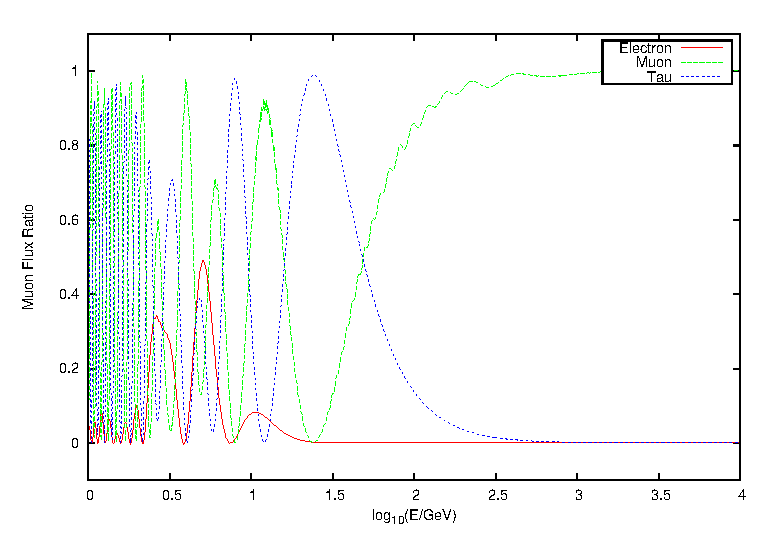
\includegraphics[width=0.7\textwidth]{fig/Multiplot.eps} 
  \caption{Output for the multiple energy mode with sterile neutrino (3+1)} 
\end{figure}
 
In fig.\ref{fig:multimode} we show the plot produced by the plotting
script for the case with sterile neutrino (3+1).


\subsection{Read and Write \textnormal{({\ttf examples/HDF5\_Write\_Read})}}

In this example we basically illustrate the use of the functions to
read and write {\ttf .hdf5} files. The content of the file is the full
information in the system, that means all the configuration
parameters, body, track, position in the track and also all the
density matrix information. This allows for example to save the system
in the middle of the propagation and read it later to keep
evolving. Another important fact is that if we save the system using
this when we read it again we can compute any quantum mechanical
observable for the saved density matrix.

This example is basically the same as the multiple energy example by
splited in two parts, one that computes the evolution ans save the
state of the system ({\ttf write.cpp}) and another that reads the
state and extract the flavor fluxes and put them in a text file ({\ttf
  read.cpp}).

In the following we will show the lines to save and load the hdf5
files.

In the file {\ttf write.cpp} we save the system before and after the
evolution.
\begin{lstlisting}[frame=leftline, numbers =
  left,breaklines=true,label = ex:sin1]
  nus.WriteStateHDF5(``./initial_state.hdf5'');
  nus.EvolveState();
  nus.WriteStateHDF5(``./final_state.hdf5'');
\end{lstlisting}

And in order to recover that in the {\ttf read.cpp} file we use the
constructor that construct directly the object for a given file name.

\begin{lstlisting}[frame=leftline, numbers =
  left,breaklines=true,label = ex:sin1]
  nuSQUIDS inus(``./initial_state.hdf5'');
  nuSQUIDS fnus(``./final_state.hdf5''); 
\end{lstlisting}


\subsection{Use and Construct Bodies \textnormal{({\ttf
      examples/Bodies})}}
One of the main classes in the nuSQUIDS library is the body and track
classes, these have to be always defined since they define the media
where the neutrinos will propagate. 
In this example we show how to use the objects already implemented in
the library and also how to create some objects from the classes
already defined.

In the folder {\ttf examples/Bodies/} the {\ttf main.cpp} file
contains the main function of the examples, that uses all the already
existing objects in nuSQUIDS and the example new modified object
defined in the heather and implementation files {\ttf exBody.h} and
{\ttf exBody.cpp}.

\subsubsection{Construct a derived Body}

Here is an example of hot to define a derived object for the EarthAtm
body, in this simple case the object is just an earth model with some
parameters that weight the relative densities in the different layers
of the earth, inner core, outer core, and mantel.

In order to implement that we have to be in the {\ttf nusquids} namespace and we define a
new class called {\ttf EarthMod} which is a derived class of {\ttf
  EarthAtm}, this means this new class we have all the properties,
values and function of the other class. 
\begin{lstlisting}[frame=leftline, numbers = left,breaklines=true,label = ex:sin1]

namespace nusquids{

class EarthMod: public EarthAtm{
public:
\end{lstlisting}
Here we define the main constructors that implement the changes,
basically we weight the inner core, outer core and mantle using the
values given by, {\ttf double frho1}, {\ttf double frho2}, {\ttf
  double frho3}
\begin{lstlisting}[frame=leftline, numbers = left,breaklines=true,label = ex:sin1,firstnumber=last]
  EarthMod(){}
  EarthMod(std::string earthmodel, double frho1, double frho2 , double
  frho3);
\end{lstlisting}
The function {\ttf Mod} allows to change the parameters ones the
object is already defined.
\begin{lstlisting}[frame=leftline, numbers =
  left,breaklines=true,label = ex:sin1,firstnumber=last]

  void  Mod(double frho1, double frho2, double frho3);
};

\end{lstlisting}

\subsubsection{Use of the Bodies}

In this part we will describe what is implemented in the {\ttf
  main.cpp} file.
This file defines a nuSQUIDS object and sets different bodies and
tracks, for everyone of these it evolve the system and shows the
probabilities in the screen.
For simplicity we use the single energy mode, \ref{sec:single}, but the use of the body
and track would be exactly the same for the multiple energy case.

First we construct the nuSQUIDS object for 3 neutrinos we set the
oscillation parameters and the energy of the neutrino that we
propagate.

\begin{lstlisting}[frame=leftline, numbers =
  left,breaklines=true,label = ex:sin1]
  nuSQUIDS nus(3,neutrino);
  nus.Set_MixingAngle(0,1,0.563942);
  nus.Set_MixingAngle(0,2,0.154085);
  nus.Set_MixingAngle(1,2,0.785398);
  nus.Set_SquareMassDifference(1,7.65e-05);
  nus.Set_SquareMassDifference(2,0.00247);
  nus.Set_CPPhase(0,2,0.0);

  squids::Const units;

  nus.Set_E(10.0*units.GeV);
\end{lstlisting}

\begin{enumerate}
\item {\ttf Earth}

The first example is the {\ttf Earth} body, in this case the track is
parametrized by the baseline of the experiment. Here we define the
body and track.
\begin{lstlisting}[frame=leftline, numbers =
  left,breaklines=true,label = ex:sin1,firstnumber=last]
  double baseline = 500.0*units.km;
  std::shared_ptr<Earth> earth = std::make_shared<Earth>();
  std::shared_ptr<Earth::Track> earth_track = std::make_shared<Earth::Track>(0.0,baseline,baseline);
\end{lstlisting}
And we set the Body and Track to the nusquids object.
\begin{lstlisting}[frame=leftline, numbers =
  left,breaklines=true,label = ex:sin1,firstnumber=last]
  nus.Set_Body(earth);
  nus.Set_Track(earth_track);
\end{lstlisting}

We first set the initial state of the system, and print the state in
the screen.
\begin{lstlisting}[frame=leftline, numbers =
  left,breaklines=true,label = ex:sin1,firstnumber=last]
  marray<double,1> ini_state({3},{0,1,0});
  nus.Set_initial_state(ini_state,flavor);
  // Lets print out the initial state
  std::cout << "In state" << std::endl;
  for (double EE : nus.GetERange()){
    std::cout << EE/units.GeV << " ";
    for(int i = 0; i < 3; i++){
      std::cout << nus.EvalFlavor(i) << " ";
    }
    std::cout << std::endl;
  }

We set the numerical error and maximum step for the GSL integrator.
\begin{lstlisting}[frame=leftline, numbers =
  left,breaklines=true,label = ex:sin1,firstnumber=last]
  nus.Set_h_max( 200.0*units.km );
  nus.Set_rel_error(1.0e-12);
  nus.Set_abs_error(1.0e-12);
\end{lstlisting}

Finally we evolve the state and print in the screen the final state of
the system.
\begin{lstlisting}[frame=leftline, numbers =
  left,breaklines=true,label = ex:sin1,firstnumber=last]

  nus.EvolveState();
  std::cout << "Out state" << std::endl;
  for (double EE : nus.GetERange()){
    std::cout << EE/units.GeV << " ";
    for(int i = 0; i < 3; i++){
      std::cout << nus.EvalFlavor(i) << " ";
    }
    std::cout << std::endl;
  }
\end{lstlisting}
This last steps in the code are the same in all the examples and we
are ommiting that for the following cases, we are only going to go though the
declaration of the body an track. 
\item {\ttf EarthAtm}

In this example we use the {\ttf EarthAtm} body. In this case the
track is defined by the zenith angle of the trajectory.
\begin{lstlisting}[frame=leftline, numbers =
  left,breaklines=true,label = ex:sin1,firstnumber=last]
  double phi = acos(-1.0);
  std::shared_ptr<EarthAtm> earth_atm = std::make_shared<EarthAtm>();
  std::shared_ptr<EarthAtm::Track> earth_atm_track = std::make_shared<EarthAtm::Track>(phi);

  nus.Set_Body(earth_atm);
  nus.Set_Track(earth_atm_track);
\end{lstlisting}

\item {\ttf earth\_mod}

Case with the modified earth object we construct as a derived object
of EarthAtm. As before the track is deffined by the zenith angle of
the trajectory, in this case we construct the object and then we rescale
all the earth density by a factor $0.1$, finally we set the body an track to nuSQUIDS. 
\begin{lstlisting}[frame=leftline, numbers =
  left,breaklines=true,label = ex:sin1,firstnumber=last]
  double phi = acos(-1.0);
  std::shared_ptr<EarthMod> earth_mod = std::make_shared<EarthMod>();
  std::shared_ptr<EarthMod::Track> earth_mod_track = std::make_shared<EarthMod::Track>(phi);  
  earth_mod->Mod(0.1,0.1,0.1);

  nus.Set_Body(earth_mod);
  nus.Set_Track(earth_mod_track);
\end{lstlisting}


\item {\ttf VariableDensity}

In this case we set a variable density body and a track of $200km$
First we define the density, position and electron fraction arrays
with the corresponding values.
\begin{lstlisting}[frame=leftline, numbers =
  left,breaklines=true,label = ex:sin1,firstnumber=last]
  int N=40;

  std::vector<double> x_arr(N);
  std::vector<double> density_arr(N);
  std::vector<double> ye_arr(N);

  double size = 1000.0*units.km;
  for(int i = 0; i < N; i++){
    x_arr[i] = size*(i/(double)N);
    density_arr[i] = fabs(cos((double)i));
    ye_arr[i] = fabs(sin((double)i));
  }
\end{lstlisting}

Now we construct the body and the track using, the constructor for the
variable density takes as an input the vectors with the
values. Finally like before we set the body ant the track to nuSQUIDS.
\begin{lstlisting}[frame=leftline, numbers =
  left,breaklines=true,label = ex:sin1,firstnumber=last]

  std::shared_ptr<VariableDensity> vardens = std::make_shared<VariableDensity>(x_arr,density_arr,ye_arr);
  std::shared_ptr<VariableDensity::Track> track_vardens = std::make_shared<VariableDensity::Track>(0.0,200.0*units.km);

  nus.Set_Body(vardens);
  nus.Set_Track(track_vardens);
\end{lstlisting}

\item {\ttf Vacuum}

This is a trivial case where the density and electron fraction are
zero, we only need to give the baseline as an argument to construct
the track. In the example we set the baseline to $500km$.

\begin{lstlisting}[frame=leftline, numbers =
  left,breaklines=true,label = ex:sin1,firstnumber=last]
  double baseline_2 = 500.0*units.km;
  std::shared_ptr<Vacuum> vacuum = std::make_shared<Vacuum>();
  std::shared_ptr<Vacuum::Track> track_vac = std::make_shared<Vacuum::Track>(baseline_2);
  
  nus.Set_Body(vacuum);
  nus.Set_Track(track_vac);
\end{lstlisting}

\item {\ttf ConstantDensity}

Case with constant density, in this case a analytic approximation is
used to propagate the neutrinos, the full Hamiltonian of the system is
diagonalized and exponentiated. This allows to solve very fast the
oscillations even when the matter potential is large.

We set the density to $100g/cm^3$ the electron fraction to 0.3 and the
baseline for the propagation to $500km$.
\begin{lstlisting}[frame=leftline, numbers =
  left,breaklines=true,label = ex:sin1,firstnumber=last]

  double density = 100.0;
  double ye = 0.3;
  std::shared_ptr<ConstantDensity> constdens = std::make_shared<ConstantDensity>(density,ye);
  double baseline_3 = 500.0*units.km;
  std::shared_ptr<ConstantDensity::Track> track_constdens =   std::make_shared<ConstantDensity::Track>(0.0,baseline_3);

  nus.Set_Body(constdens);
  nus.Set_Track(track_constdens);
\end{lstlisting}

Notice that the system sets the nusquids in the mass basis in order to
do the approximation, that can produce problems in the future uses of
the same nuSQUIDS object.

\end{enumerate}


\subsection{ Cross Sections \textnormal{({\ttf
      examples/Xsections})}}

One of the strong sides of nuSquids is the possibility of adding in a
consistent way the non coherent interaction, the physical quantity
that encodes how often this scattering interaction are happening
between the neutrinos and the media is the cross section and is all in
the cross section class.

In this example we show a very basic extension of the standard
cross section class in a way that extends the values to low energies, 
in the region where the cross section can be very well approximated by
zero.

The new derived class for the extended cross section is in the header
{\ttf exCross.h} and the implementation file {\ttf exCross.cpp}, the
main file is an example using this new cross section in the multiple
energy mode.

The new derived class {\ttf
  NeutrinoDISCrossSectionsFromTablesExtended} its just the same class
as {\ttf NeutrinoDISCrossSectionsFromTables} but returning zero for
the Total and differential cross sections when the energy is lower
than the lowest energy in the tables.

Here we define the constructor, the {\ttf TotalCrossSection} and {\ttf SingleDifferentialCrossSection}
\begin{lstlisting}[frame=leftline, numbers =
  left,breaklines=true,label = ex:sin1]
  
  class NeutrinoDISCrossSectionsFromTablesExtended : public NeutrinoDISCrossSectionsFromTables {
    public :
    NeutrinoDISCrossSectionsFromTablesExtended():NeutrinoDISCrossSectionsFromTables(){}
    double TotalCrossSection(double Enu, NeutrinoFlavor flavor, NeutrinoType neutype, Current current) const override;
    double SingleDifferentialCrossSection(double E1, double E2, NeutrinoFlavor flavor, NeutrinoType neutype, Current current) const override;
  };
 
\end{lstlisting}

The implementation file is just.
\begin{lstlisting}[frame=leftline, numbers =
  left,breaklines=true,label = ex:sin1]
  double NeutrinoDISCrossSectionsFromTablesExtended::TotalCrossSection(
  double Enu, NeutrinoFlavor flavor, NeutrinoType neutype, Current current) const{
    if (not (flavor == electron or flavor == muon or flavor == tau))
      return 0.0;
    if (Enu < Emin)
      return std::numeric_limits<double>::min();
    else
      return NeutrinoDISCrossSectionsFromTables::TotalCrossSection(Enu, flavor, neutype, current);
  }
  
  double NeutrinoDISCrossSectionsFromTablesExtended::SingleDifferentialCrossSection(double
  E1, double E2, NeutrinoFlavor flavor, NeutrinoType neutype, Current current) const{
    if (not (flavor == electron or flavor == muon or flavor == tau))
      return 0.0;
    if (E1 < Emin || E2<Emin)
      return std::numeric_limits<double>::min();
    else
      return NeutrinoDISCrossSectionsFromTables::SingleDifferentialCrossSection(E1, E2, flavor, neutype, current);
  }
 
\end{lstlisting}

In order to use that in the main function we construct the new cross
section object and construct the nusquids using that.

\begin{lstlisting}[frame=leftline, numbers =
  left,breaklines=true,label = ex:sin1]
  std::shared_ptr<NeutrinoCrossSections> ncs=std::make_shared<NeutrinoDISCrossSectionsFromTablesExtended>();
  nuSQUIDS nus(Emin,Emax,200,numneu,neutrino,true,true,ncs);
\end{lstlisting}


\begin{figure}[h!]
  \label{fig:crossext}
  \centering
  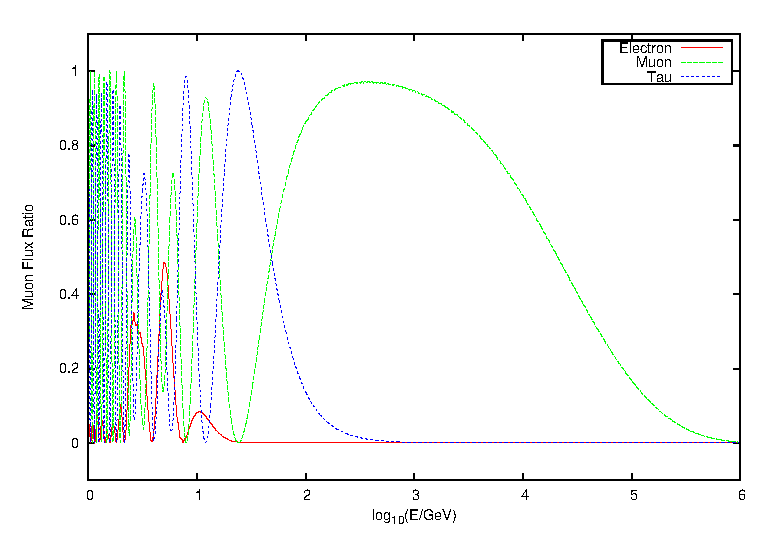
\includegraphics[width=0.7\textwidth]{fig/crossext.eps} 
  \caption{New low energy extended cross sections example} 
\end{figure}



\subsection{ Constant Density Layers \textnormal{({\ttf
      examples/Constant\_density\_layers})}}
Since the constant density allows us to do very fast computation using
the diagonalization of the full Hamiltonian here we show an example
where we concatenate the evolution of the neutrinos through different
layers of constant density.

First we construct the different layers, the first is $100km$ in
vacuum, the second $50km$ in matter with density $3.5g/cm^3$ and
$y_e=0.5$ and finally $200km$ in matter with density $10g/cm^3$ and
$y_e=0.1$.
\begin{lstlisting}[frame=leftline, numbers =
  left,breaklines=true,label = ex:sin1]

  const double layer_1 = 100.*units.km;
  std::shared_ptr<Vacuum> vacuum = std::make_shared<Vacuum>();
  std::shared_ptr<Vacuum::Track> track_env0 = std::make_shared<Vacuum::Track>(layer_1);

  const double layer_2 = 50.*units.km;
  std::shared_ptr<ConstantDensity> constdens_env1 = std::make_shared<ConstantDensity>(3.5,0.5); 
  std::shared_ptr<ConstantDensity::Track> track_env1 = std::make_shared<ConstantDensity::Track>(layer_2);

  const double layer_3 = 200.*units.km;
  std::shared_ptr<ConstantDensity> constdens_env2 = std::make_shared<ConstantDensity>(10.,0.1);
  std::shared_ptr<ConstantDensity::Track> track_env2 = std::make_shared<ConstantDensity::Track>(layer_3);

\end{lstlisting}

Now in order to evolve the system, we should set the corresponding body
and track and evolve every layer.
\begin{lstlisting}[frame=leftline, numbers =
  left,breaklines=true,label = ex:sin1]

  nus.Set_Body(vacuum);
  nus.Set_Track(track_env0);
  nus.EvolveState();


  nus.Set_Body(constdens_env1);
  nus.Set_Track(track_env1);
  nus.EvolveState();

  nus.Set_Body(constdens_env2);
  nus.Set_Track(track_env2);
  nus.EvolveState();

\end{lstlisting}

Finally we write the output for the different fluxes in flavor in a text file.

\subsection{ Non Standard Neutrino Interaction \textnormal{({\ttf
      examples/NSI})}}
Neutrino oscillations are a good probe for new physics, in this
example we illustrate an example of constructing a derived class of
nusquids in order to add some new physics modification, similarly can
be done in any other new physics scenario.

The implementation of the {\ttf nuSQUIDSNSI} is done in {\ttf NSI.h}.
First we will go trough the implementation to see what needs to be
added to be base class nuSQUIDS.
Some new variables are needed to implement the NSI matter potential,
We declare a {\ttf SU\_vector} called {\ttf NSI} that is the matter
potential, because we are working in the interaction picture we need
to define a matter potential that is accordingly rotated with $H_0$ for
every energy, this would be stored in {\ttf NSI\_evol}.
{\ttf HI\_prefactor} contains all the numerical factor in front of the
operator and {\ttf epsilon\_mutau} is the strength of the NSI non flavor
diagonal term, notice that we have the NSI diagonal contribution to
zero.

\begin{lstlisting}[frame=leftline, numbers =
  left,breaklines=true,label = ex:sin1]

class nuSQUIDSNSI: public nuSQUIDS {
  private:
    squids::SU_vector NSI;
    std::vector<squids::SU_vector> NSI_evol;
    std::unique_ptr<double[]> hiBuffer;
    double HI_prefactor;
    // nsi parameters
    double epsilon_mutau;

\end{lstlisting}

Before computing any derivative or r.h.s of the differential equation
we should have the NSI operator in the interaction picture. We add
this in prederive.
\begin{lstlisting}[frame=leftline, numbers =
  left,breaklines=true,label = ex:sin1,firstnumber=last]

    void AddToPreDerive(double x){
      for(int ei = 0; ei < ne; ei++){
        NSI_evol[ei] = NSI.Evolve(H0_array[ei],(x-Get_t_initial()));
      }
    }

\end{lstlisting}

This functions are auxiliary functions that allow the nuSQuIDSNSI to
save all the new information that defines the new derived object in
the hdf5 files.

\begin{lstlisting}[frame=leftline, numbers =
  left,breaklines=true,label = ex:sin1,firstnumber=last]

    void AddToReadHDF5(hid_t hdf5_loc_id){
      // here we read the new parameters now saved in the HDF5 file
      hid_t nsi = H5Gopen(hdf5_loc_id, "nsi", H5P_DEFAULT);
      H5LTget_attribute_double(hdf5_loc_id,"nsi","mu_tau" ,&epsilon_mutau);
      H5Gclose(nsi);
    }

    void AddToWriteHDF5(hid_t hdf5_loc_id) const {
      // here we write the new parameters to be saved in the HDF5 file
      H5Gcreate(hdf5_loc_id, "nsi", H5P_DEFAULT, H5P_DEFAULT, H5P_DEFAULT);
      H5LTset_attribute_double(hdf5_loc_id, "nsi","mu_tau",&epsilon_mutau, 1);
    }

\end{lstlisting}

And probably the most important part, where we compute the value of
the matter potential i.e. {\ttf HI}, notice at the end the different
sign for neutrinos and antineutrinos.
\begin{lstlisting}[frame=leftline, numbers =
  left,breaklines=true,label = ex:sin1,firstnumber=last]

    squids::SU_vector HI(unsigned int ei,unsigned int index_rho) const{
      double CC = HI_prefactor*body->density(*track)*body->ye(*track);


      squids::SU_vector potential(nsun,hiBuffer.get());

      potential = (3.0*CC)*NSI_evol[ei];

      if ((index_rho == 0 and NT==both) or NT==neutrino){
          return nuSQUIDS::HI(ei,index_rho) + potential;
      } else if ((index_rho == 1 and NT==both) or NT==antineutrino){
          return nuSQUIDS::HI(ei,index_rho) + (-1.0)*std::move(potential);
      } else{
          throw std::runtime_error("nuSQUIDS::HI : unknown particle or antiparticle");
      }
    }

\end{lstlisting}

In the public function we have the constructor, first calls the
nuSQUIDS constructor and after sets up the standard oscillation
paramters and the NSI operator.  
\begin{lstlisting}[frame=leftline, numbers =
  left,breaklines=true,label = ex:sin1,firstnumber=last]

  public:
  nuSQUIDSNSI(double epsilon_mutau, double Emin,double Emax,int Esize,int numneu, NeutrinoType NT,
	      bool elogscale,bool iinteraction,double th01=0.563942, double th02=0.154085, 
	      double th12=0.785398) : nuSQUIDS(Emin,Emax,Esize,numneu,NT,elogscale,iinteraction),
				      hiBuffer(new double[nsun*nsun]),epsilon_mutau(epsilon_mutau)
  {
    assert(numneu == 3);
    // defining a complex matrix M which will contain our flavor
    // violating flavor structure.
    gsl_matrix_complex * M = gsl_matrix_complex_calloc(3,3);
    gsl_complex c {{ epsilon_mutau , 0.0 }};
    gsl_matrix_complex_set(M,2,1,c);
    gsl_matrix_complex_set(M,1,2,gsl_complex_conjugate(c));
    
    NSI = squids::SU_vector(M);
    
    Set_MixingAngle(0,1,th01);
    Set_MixingAngle(0,2,th02);
    Set_MixingAngle(1,2,th12);
    
    // rotate to mass reprentation
    NSI.RotateToB1(params);
    NSI_evol.resize(ne);
    for(int ei = 0; ei < ne; ei++){
      NSI_evol[ei] = squids::SU_vector(nsun);
    }
    gsl_matrix_complex_free(M);
    
    HI_prefactor = params.sqrt2*params.GF*params.Na*pow(params.cm,-3);
  }

\end{lstlisting}

This last function set the value of {\ttf epsilon\_mutau}, changing the
value of the {\ttf SU\_vector NSI} accordingly 

\begin{lstlisting}[frame=leftline, numbers =
  left,breaklines=true,label = ex:sin1,firstnumber=last]
  
  void Set_mutau(double eps){
    gsl_matrix_complex * M = gsl_matrix_complex_calloc(3,3);
    gsl_complex c {{ epsilon_mutau , 0.0 }};
    gsl_matrix_complex_set(M,2,1,c);
    gsl_matrix_complex_set(M,1,2,gsl_complex_conjugate(c));
    NSI = squids::SU_vector(M);    
    NSI.RotateToB1(params);
    gsl_matrix_complex_free(M);
  }
 
  
\end{lstlisting}


In the main function in {\ttf main.cpp} we use the new NSI in a
multiple energy mode. In order
to see the effect of having NSI we propagate the case with {\ttf
  epsilon\_mutau=0} and {\ttf epsilon\_mutau=1e-2}.


\begin{lstlisting}[frame=leftline, numbers =
  left,breaklines=true,label = ex:sin1,firstnumber=last]

  double eps_mutau=1.0e-2;
  nuSQUIDSNSI nus(eps_mutau,Emin,Emax,200,numneu,antineutrino,true,false);
  nuSQUIDSNSI nus_zero(0.0,Emin,Emax,200,numneu,antineutrino,true,false);
\end{lstlisting}

After setting all the parameters we propagate both cases, and put both
fluxes in a text file.

\begin{lstlisting}[frame=leftline, numbers =
  left,breaklines=true,label = ex:sin1,firstnumber=last]

  nus.EvolveState();
  nus_zero.EvolveState();

  int Nen =1000;
  double lEmin=log10(Emin);
  double lEmax=log10(Emax);
  
  std::ofstream file("fluxes_flavor.txt");

  file << "# log10(E) E flux_NSI_i flux_noNSI_i . . . ." << std::endl;
  for(double lE=lEmin; lE<lEmax; lE+=(lEmax-lEmin)/(double)Nen){
    double E=pow(10.0,lE);
    file << lE << " " << E << " ";
    for(int fl=0; fl<numneu; fl++){
      file << " " <<  nus.EvalFlavor(fl, E) << " " <<  nus_zero.EvalFlavor(fl, E);
    }
    file << std::endl;
  }

\end{lstlisting}

In the folder there is a script that allows to plot the output text
file.

\subsection{ Atmospheric Mode \textnormal{({\ttf
      examples/Atm\_default})}}
In this example we show how to use the atmospheric mode, this mode is
compact way to treat set of nuSQUIDS objects distributed in zenith, this
allows us to treat the problem of
propagating the full, energy and zenith dependent, atmospheric neutrino flux trough the earth.

First we construct the nuSQUIDSAtm object. The paremeters we are
setting is the range of cosine of the zenith angle from $-1$ to $0.2$
and in energies from $10GeV$ to $1e6GeV$, we chose 40 nodes in zenith.
Notice that the parameters after the zenith information are the same
than the basic nuSQUIDS object.

\begin{lstlisting}[frame=leftline, numbers =
  left,breaklines=true,label = ex:sin1]

  double Emin=1.e1*units.GeV;
  double Emax=1.e6*units.GeV;
  double czmin=-1;
  double czmax=0;

  nuSQUIDSAtm<> nus_atm(czmin,czmax,40,Emin,Emax,100,numneu,both,true,interactions);

\end{lstlisting}

In this case we have to give the initial state also depending on
zenith, here we fill the array with and set the initial state of the
system. The function {\ttf flux\_function} would be the corresponding
atmospheric flux.

\begin{lstlisting}[frame=leftline, numbers =
  left,breaklines=true,label = ex:sin1,firstnumber=last]

  marray<double,4> inistate{nus_atm.GetNumCos(),nus_atm.GetNumE(),2,numneu};
  std::fill(inistate.begin(),inistate.end(),0);
  for ( int ci = 0 ; ci < nus_atm.GetNumCos(); ci++){
    for ( int ei = 0 ; ei < nus_atm.GetNumE(); ei++){
      for ( int rho = 0; rho < 2; rho ++ ){
        for (int flv = 0; flv < numneu; flv++){
          inistate[ci][ei][rho][flv] = (flv == 1) ? flux_function(e_range[ei], cz_range[ci]) : 0.0;//set 1 only to the muon flavor
        }
      }
    }
  }

  nus_atm.Set_initial_state(inistate,flavor);

\end{lstlisting}


To evolve the full state we call

\begin{lstlisting}[frame=leftline, numbers =
  left,breaklines=true,label = ex:sin1,firstnumber=last]

nus_atm.EvolveState();

\end{lstlisting}

Finally we save the flux in a output text file, notice that the
atmospheric mode has an interpolation implemented, therefore you can
evaluate the flux at any flavor, energy, and zenith. See \ref{sec:atm}
for more details.
\ref{sec:atm}.

\begin{lstlisting}[frame=leftline, numbers =
  left,breaklines=true,label = ex:sin1,firstnumber=last]

  int Nen=700;
  int Ncz=100;
  double lEmin=log10(Emin);
  double lEmax=log10(Emax);;

  file << "# log10(E) cos(zenith) E flux_i . . . ." << std::endl;
  for(double cz=czmin;cz<czmax;cz+=(czmax-czmin)/(double)Ncz){
    for(double lE=lEmin; lE<lEmax; lE+=(lEmax-lEmin)/(double)Nen){
      double E=pow(10.0,lE);
      file << lE << " " << cz << " " << E;
      for(int fl=0; fl<numneu; fl++){
	file << " " <<  nus_atm.EvalFlavor(fl,cz, E);
      }
      file << std::endl;
    }
    file << std::endl;
  }

\end{lstlisting}



\subsection{ Atmospheric With Derived nuSQUIDS Class \textnormal{({\ttf
      examples/Atm\_NSI})}}

The Atmospheric mode is done in a way that can be used not only with
the basic nuSQUIDS class but also with derived classes. In this
example we use the atmospheric mode but with the NSI nuSQUIDS
extension shown in the NSI example.

In the folder we add the {\ttf NSI.h} file, this file is exactly the
same as in the NSI example, and the main file is essentially the same as
the atmospheric default mode example with the following changes.

\begin{lstlisting}[frame=leftline, numbers =
  left,breaklines=true,label = ex:sin1,firstnumber=last]

  double epsilon_mutau=1e-2;
  nuSQUIDSAtm<nuSQUIDSNSI> nus_atm(czmin,czmax,40,epsilon_mutau,Emin,Emax,100,numneu,both,true,true);

\end{lstlisting}

notice that in this example the arguments are always, first the zenith
arguments {\ttf czmin, czmax, 40} and second the arguments of the
nuSQUIDS derive object, in this case for the NSI {\ttf
  epsilon\_mutau,Emin,Emax,100,numneu,both,true,true}. This structure
will hold for any derive nuSQUIDS class.


 

\section{Performance, and precision}

\section{Test suite}

\section{Description of the code} 
\label{sec:code} 

$\nu$-SQuIDS is a {\ttf C++} code built using the SQuIDS
framework \citep{SQUIDS}. It is designed to propagate neutrinos
through media while taking into account flavor oscillations and
noncoherent interactions. 

In order to allow the user to compute simple oscillation probabilities
for a single energy the code has a simplified mode.
In this mode the neutrino energy is fixed and only coherent interactions
are treated.
In this case, only Eq. \eqref{eq:schrodinger} is relevant for the
neutrino propagation, and the {\ttf nuSQuIDS} class implements {\ttf
  SQuIDS::H0} as in Eq. \eqref{eq:h0} and {\ttf SQuIDS::HI} as given
in Eq. \eqref{eq:hi}. 

In the default mode a statistical ensemble of neutrinos is
considered. The ensemble is described by means of a set of {\ttf
  SU\_vector} objects located at fixed  energy nodes spaced over the
energy region under consideration. Besides defining {\ttf SQuIDS::H0}
and {\ttf SQuIDS::HI}, as in the simplified single energy mode, the
following functions are also defined: {\ttf SQuIDS::GammaRho} by
equations \eqref{eq:gammarhoa} and \eqref{eq:gammarhob}, and {\ttf
  SQuIDS::InteractionsRho} in equations \eqref{eq:Fterm} and
\eqref{eq:antiFterm}. Furthermore, in the latter equation
\eqref{eq:antiFterm} $\tau$-regeneration is implemented assuming
instantaneous $\tau$ decay.

While the {\ttf nuSQuIDS} class implements all the necessary
differential equations, one must also specify the neutrino propagation
environment, propagation trajectory, and the relevant cross sections.  
When interactions are considered the {\ttf nuSQuIDS} instance
will automatically construct appropriate {\ttf NeutrinoCrossSections}
and {\ttf TauDecaySpectra} objects to evaluate cross sections and
$\tau$ physics respectively, however, the user can also replace these
default versions if desired. On the other hand, the user must
explicitly specify the neutrino propagation medium and trajectory
through relevant specialization of {\ttf Body} and {\ttf Body::Track}.
Several implementations of {\ttf Body} and {\ttf Track} covering
common physics cases are supplied with the library. 

Finally, {\ttf nuSQuIDS} provides a set functions to evaluate the
neutrino ensemble flavor and mass composition as well as the
capability to store the system state in an HDF5 \citep{folk1999hdf5}
file for later use.

% TODO: mention setting mixing parameters used for propagation

\subsection{Body \& Track}

{\ttf Body} and {\ttf Body::Track} are abstract {\ttf C++} classes
which are used to represent the environment in which neutrinos
are propagated ({\ttf Body}) and the propagation path inside it ({\ttf
  Body::Track}). We will frequently use the shorthand {\ttf Track} for {\ttf Body::Track},
 when it should be clear from context that this is the type of {\ttf Track} 
 corresponding to a particular implementation of {\ttf Body}.

The evolution of the system depends on a single parameter which is
{\ttf double} member of {\ttf Track}. The
interplay between the evolution of this parameter and the trajectory
inside a given body is what is encoded in the {\ttf Body} and 
{\ttf Body::Track} classes. 
Namely, a {\ttf Body} is defined as a matter density and electron
fraction depending on the position in a 3 dimensional space, $\rho_m(\vec{r})$ and
$Y_e(\vec{r})$, the role of the {\ttf Track} would be
equivalent to the trajectory ($\vec{r}(x)$) and the current position ($x$).

In the context of the code, the two main virtual functions that the
user should provide in order to define a non-trivial {\ttf Body} are:
\begin{itemize}
\item[$\circ$] 
  \begin{lstlisting}
    virtual double density(std::shared_ptr<Track>);
  \end{lstlisting}
This function returns the density in ${\rm g}/{\rm cm}^3$ for a
given {\ttf Track} position.
\item[$\circ$] 
  \begin{lstlisting}
    virtual double ye(std::shared_ptr<Track>);
  \end{lstlisting}
Returns the electron fraction at a given {\ttf Track} position.
\end{itemize}

In order to allow the user to store the information of the
object the following members are important,

\begin{itemize}
\item[$\circ$]  
  \begin{lstlisting}
    std::vector<double> BodyParams;
  \end{lstlisting}
  Double vector that contains all the parameters that are
  needed to compute the density and electron fraction from the parameter
  {\ttf x}.
  
\item[$\circ$]  
  \begin{lstlisting}
    bool is_constant_density = false;
  \end{lstlisting}  
  This variable is {\ttf true} if the density of the object is constant. This is
  used to set the fast computations internally.
\end{itemize}

Other public function of the {\ttf Body} object are,

\begin{itemize}
\item[$\circ$]  
  \begin{lstlisting}
    virtual void Serialize(hid_t group) const=0;
  \end{lstlisting}
  This is an abstract function whose argument is an HDF5 location
  where the user should store the body properties.

  \item[$\circ$]  
  \begin{lstlisting}
    static std::shared_ptr<Body> Deserialize(hid_t group);
  \end{lstlisting}
  This is an abstract function whose argument is an HDF5 location
  with the body information to be used for the user to recover the body.
  
\item[$\circ$]  
  \begin{lstlisting}
    unsigned int GetId() const {return 0;}
  \end{lstlisting}
  It returns the Id of the body which is hard coded by the user.

\item[$\circ$]  
  \begin{lstlisting}
    std::string GetName() const {return name;}
  \end{lstlisting}
  It returns the name of the object which is hard coded by the user.

\item[$\circ$]  
  \begin{lstlisting}
    const std::vector<double>& GetBodyParams() const { return BodyParams;}
  \end{lstlisting}
  It returns a constant reference to the vector of parameter that define body. 
  
  \item[$\circ$]  
  \begin{lstlisting}
    virtual bool IsConstantDensity() const {return is_constant_density;}
  \end{lstlisting}
  It returns true or false if its a constant density body.
  
\item[$\circ$]  
  \begin{lstlisting}
    virtual void SetIsConstantDensity(bool icd) {is_constant_density = icd;}
  \end{lstlisting}
  Set true or false the constant density. 
\end{itemize}


Furthermore, the {\ttf Track} object has the following protected
variables, which are the initial, final and current
evolution parameter values, by default in units of eV$^{-1}$
%
%
\begin{itemize}
\item[$\circ$]  
  \begin{lstlisting}
  double x;
  \end{lstlisting}
  Current position.
\item[$\circ$]  
  \begin{lstlisting}
    double xini;
  \end{lstlisting}
  Initial position.
\item[$\circ$]  
  \begin{lstlisting}
    double xend;
  \end{lstlisting}
  Final position.
\end{itemize}
%
And the following public functions are provided,
%
\begin{itemize}
\item[$\circ$]  
  \begin{lstlisting}
    Track(double x,double xini, double xend): x(x), xini(xini),xend(xend) {}
  \end{lstlisting}
  Constructor where we specify current, initial, and final positions. 
\item[$\circ$]  
  \begin{lstlisting}
    Track(double xini, double xend): Track(xini,xini,xend) {}
  \end{lstlisting}
  Constructor where we specify initial and final positions. The
  current position is set to the initial. 
  \item[$\circ$]  
  \begin{lstlisting}
    virtual void Serialize(hid_t group) const=0;
  \end{lstlisting}
  This is an abstract function whose argument is an HDF5 location
  where the user should store the track properties.
  \item[$\circ$]  
  \begin{lstlisting}
    static std::shared_ptr<Body::Track> Deserialize(hid_t group);
  \end{lstlisting}
  This is an abstract function whose argument is an HDF5 location
  with the track information to be used for the user to recover the track.
\item[$\circ$]  
  \begin{lstlisting}
    void SetX(double y);
  \end{lstlisting}
  Sets the current position along the trajectory.  
\item[$\circ$]  
  \begin{lstlisting}
    double GetX() const;
  \end{lstlisting}
  Returns the current value of the evolution parameter {\ttf x}.
\item[$\circ$]  
  \begin{lstlisting}
    double GetInitialX() const;
  \end{lstlisting}    
  Returns the initial value of the evolution parameter {\ttf x}.
\item[$\circ$]  
  \begin{lstlisting}
    double GetFinalX() const;
  \end{lstlisting}          
  Returns the final value of the evolution parameter {\ttf x}
\item[$\circ$]  
  \begin{lstlisting}
    static std::string GetName() {return "BodyTrack";};
  \end{lstlisting}
  Returns the name of the track object hard coded by the user. 
\item[$\circ$]  
  \begin{lstlisting}
    std::vector<double> GetTrackParams() const 
  \end{lstlisting}           
  Returns a vector of doubles that define the trajectory.
\item[$\circ$] 
   \begin{lstlisting}
    virtual void FillDerivedParams(std::vector<double>& TrackParams) const{};
  \end{lstlisting}           
  Should be implemented by derived classes to append their
  additional parameters to TrackParams
  
\item[$\circ$] 
  \begin{lstlisting}
    void ReverseTrack() 
  \end{lstlisting}
  Interchanges initial and final positions.
\end{itemize}


Since {\ttf Body} and {\ttf Track} are abstract classes they themselves do not perform any task, but rather their specializations specify the real neutrino propagation environment and how it relates to its trajectory. $\nu$-SQuIDS implements the most commonly used environments and trajectory configurations. The user can create new classes in order to extend $\nu$-SQuIDS functionality.

The {\ttf Body} classes specializations implemented in $\nu$-SQuIDS
are the following: {\ttf Vacuum}, {\ttf ConstantDensity}, {\ttf
  VariableDensity}, {\ttf Earth}, {\ttf EarthAtm}, {\ttf Sun}, and {\ttf SunASnu}.

In the following sub-sections we will describe the specific
constructors and the functions that are not member of the parent class.

\subsubsection{Vacuum}

\begin{itemize}
\item[$\circ$] {\ttf Vacuum}
  \begin{lstlisting}
    Vacuum():Body(){}
  \end{lstlisting}
  Initializes a {\ttf Vacuum} environment. 
\item[$\circ$] {\ttf Vacuum::Track}
  \begin{lstlisting}
        Track(double x,double xini,double xend):Body::Track(x,xini,xend){};
        Track(double xini,double xend):Track(xini,xini,xend){};
        Track(double xend):Track(0.0,xend){}
  \end{lstlisting}
  Initialize the corresponding {\ttf Track} setting the current ({\ttf
  x}), initial ({\ttf xini}), and final ({\ttf xend}) neutrino position in ${\rm eV}^{-1}$.
\end{itemize}

\subsubsection{ConstantDensity}

\begin{itemize}
\item[$\circ$] {\ttf ConstantDensity}
  \begin{lstlisting}
    ConstantDensity(double density,double ye);
  \end{lstlisting}
  Initializes a {\ttf ConstantDensity} environment with constant
  density ({\ttf density} in ${\rm g}/{\rm cm}^3$) and electron
  fraction ({\ttf ye}).
\item[$\circ$] {\ttf ConstantDensity::Track}
  \begin{lstlisting}
    Track(double x,double xini,double xend):Body::Track(x,xini,xend){};
    Track(double xini,double xend):Track(xini,xini,xend){};
    Track(double xend):Track(0.0,xend){}
  \end{lstlisting}
  Initialize the corresponding {\ttf Track} setting the current ({\ttf
  x}), initial ({\ttf xini}), and final ({\ttf xend}) neutrino position in ${\rm eV}^{-1}$.
\end{itemize}

\subsubsection{VariableDensity}

\begin{itemize}
\item[$\circ$] {\ttf VariableDensity}
  \begin{lstlisting}
    VariableDensity(std::vector<double> x,std::vector<double> density,
    std::vector<double> ye);
  \end{lstlisting}
  Initializes a {\ttf VariableDensity} environment given three equal size arrays specifying the density and electron fraction at given positions. An object will be created that interpolates using {\ttfamily gsl\_spline} \citep{gough2009gnu} along the {\ttf x} array to get the density and electron fraction as continuous functions.
  \item[$\circ$] {\ttf VariableDensity::Track}
  \begin{lstlisting}
    Track(double x,double xini,double xend):Body::Track(x,xini,xend){};
    Track(double xini,double xend):Track(xini,xini,xend){};
    Track(double xend):Track(0.0,xend){}
  \end{lstlisting}
  Initialize the corresponding {\ttf Track} setting the current ({\ttf
  x}), initial ({\ttf xini}), and final ({\ttf xend}) neutrino position in ${\rm eV}^{-1}$.
\end{itemize}

\subsubsection{Earth}
The {\ttf Earth} body specification is designed to propagate neutrinos
in the earth form two points in the surface, since the earth in the
PREM model is assumed to be spherically symmetric the length of the
path is enough to determine the trajectory. {\ttfamily AkimaSpline}~\ref{sec:tools} is used to interpolate $\rho$ and $y_e$ as a function of radius to the earth center.
\begin{itemize}
\item[$\circ$] {\ttf Earth}
  \begin{lstlisting}
    Earth();
  \end{lstlisting}
  Initializes an {\ttf Earth} environment as defined by the PREM \citep{dziewonski1981preliminary}.
  \begin{lstlisting}
    Earth(std::string earthmodel);
  \end{lstlisting}
  Initializes an {\ttf Earth} environment as defined by a table given in the file specified by {\ttf filepath}. The table should have three columns: radius (where 0 is center and 1 is surface), density (${\rm g}/{\rm cm}^3$), and $y_e$ (dimensionless). 
  \begin{lstlisting}
    Earth(std::vector<double> x,std::vector<double> rho,std::vector<double> ye);
  \end{lstlisting}
  Initialize an {\ttf earth} whose radial density is specified by the
  values in the vector {\ttf rho} in ${\rm g}/{\rm cm}^3$, the
  electron fraction in the vector {\ttf ye}, and the radial positions
  in the vector {\ttf x} in centimeters. 

  \begin{lstlisting}
    double GetRadius() const;
  \end{lstlisting}
  Returns the radius of the Earth in eV$^{-1}$.

\item[$\circ$] {\ttf Earth::Track}
  \begin{lstlisting}
        Track(double x,double xini,double xend,double baseline):Body::Track(x,xini,xend),baseline(baseline){};
        Track(double xini,double xend,double baseline):Track(xini,xini,xend,baseline){};
  \end{lstlisting}
  Initialize the corresponding {\ttf Track} setting the current ({\ttf
    x}), initial ({\ttf xini}), and final ({\ttf xend}) neutrino position in ${\rm eV}^{-1}$.
  
  \begin{lstlisting}
    Track(double baseline):Track(0.,baseline,baseline){}
  \end{lstlisting}
  Constructor that sets the path on the earth for a given baseline
  {ttf baseline}

  \begin{lstlisting}
    double GetBaseline() const;
  \end{lstlisting}
  Returns the baseline in eV$^{-1}$.
    
\end{itemize}

\subsubsection{{EarthAtm}}
This is to be used when the relevant parameter is the zenith angle of
the path,
\begin{itemize}
\item[$\circ$] {\ttf EarthAtm}
  \begin{lstlisting}
    Earth();
  \end{lstlisting}
  Initializes an {\ttf Earth} environment as defined by the PREM \citep{dziewonski1981preliminary}.
  \begin{lstlisting}
    Earth(std::string earthmodel);
  \end{lstlisting}
  Initializes an {\ttf Earth} environment as defined by a table given in the file specified by {\ttf filepath}. The table should have three columns: radius (where 0 is center and 1 is surface), density (${\rm g}/{\rm cm}^3$), and $y_e$ (dimensionless). 
  \begin{lstlisting}
    Earth(std::vector<double> x,std::vector<double> rho,std::vector<double> ye);
  \end{lstlisting}
  Initialize an {\ttf earth} whose radial density is specified by the
  values in the vector {\ttf rho} in ${\rm g}/{\rm cm}^3$, the
  electron fraction in the vector {\ttf ye}, and the radial positions
  in the vector {\ttf x} in centimeters. 

\item[$\circ$] {\ttf EarthAtm::Track}
  \begin{lstlisting}
    Track(double x_,double phi):Track(phi){x=x_;};
    Track(double phi);
  \end{lstlisting}
  Initialize the corresponding {\ttf Track} by specifying the zenith
  angle in radians ({\ttf phi}) and the current position along the
  track ({\ttf x}) in eV$^{-1}$.
  
  \begin{lstlisting}
    double GetBaseline() const;
  \end{lstlisting}
  Returns the baseline in eV$^{-1}$.

  \begin{lstlisting}
    static Track makeWithCosine(double cosphi);
  \end{lstlisting}
  Initialize the track with the cosine of the zenith angle ({\ttf cosphi}) instead. 
  
\end{itemize}

\subsubsection{{Sun}}
This specification of the object allows to define the Sun and radial
trajectories that start from the center of the sun.
\begin{itemize}
\item[$\circ$] {\ttf Sun}
  \begin{lstlisting}
    Sun();
  \end{lstlisting}
  Initializes an {\ttf Sun} environment as defined by the {\it
    Standard Solar Model}~\citep{bahcall2005new}.
  
  \begin{lstlisting}
    Sun(std::vector<double> x,std::vector<double>
    rho,std::vector<double> xh);
  \end{lstlisting}
  Initialize an {\ttf Sun} whose radial density is specified by the
  values in the vector {\ttf rho} in ${\rm g}/{\rm cm}^3$, the
  electron fraction in the vector {\ttf ye}, and the radial positions
  in the vector {\ttf x} in centimeters. 
  
\item[$\circ$] {\ttf Sun::Track}
  \begin{lstlisting}
    Sun::Track(double xini);
  \end{lstlisting}
  This constructor sets the trajectory starting at a distance 
  {\ttf xini} from the Sun center.
  \item[$\circ$] {\ttf Sun::Track}
  \begin{lstlisting}
    Sun::Track(double xini, double xend);
  \end{lstlisting}
  Initialize the corresponding {\ttf Track} by the initial position in the sun {\ttf xini} and {\ttf xend} along the solar radius.
\end{itemize}


\subsubsection{{SunASnu}}
This specification of the object allows to define the Sun and the
trajectories with different impact parameters.
\begin{itemize}
\item[$\circ$] {\ttf Sun}
  \begin{lstlisting}
    SunASun();
  \end{lstlisting}
  Initializes an {\ttf Sun} environment as defined by the {\it
    Standard Solar Model}~\citep{bahcall2005new}.
  \begin{lstlisting}
    SunASnu(std::vector<double> x,std::vector<double> rho,
    std::vector<double> xh);
  \end{lstlisting}
  Initialize an {\ttf Sun} whose radial density is specified by the
  values in the vector {\ttf rho} in ${\rm g}/{\rm cm}^3$, the
  electron fraction in the vector {\ttf ye}, and the radial positions
  in the vector {\ttf x} in centimeters. 
  
\item[$\circ$] {\ttf SunASun::Track}
  \begin{lstlisting}
    Track(double x,double xini,double b_impact);
    Track(double xini,double b_impact):Track(xini,xini,b_impact){};
    Track(double b_impact_):Track(0.0,b_impact_){}
  \end{lstlisting}
  This constructor sets the trajectory starting at a distance 
  {\ttf xini}, with current position {\ttf x}, and impact factor {\ttf
    b\_impact} in eV$^-{1}$.
\end{itemize}

\subsection{NeutrinoCrossSections}
\label{sec:xs}
This object can be query to obtain neutrino cross section information used when considering neutrino non-coherent interactions. The {\ttf NeutrinoCrossSections} is a base abstract class, which the user has to subclass and implement the relevant neutrino cross section for the problem at hand. The user must specify the total cross section per flavor and per interaction type (charge and neutral current), as well as the single differential cross sections with respect to the outgoing neutrino energy.

\subsubsection{NeutrinoCrossSections}

First, we define enumerations to lable flavor, neutrino, and interaction type.
\begin{itemize}
  \item {\ttf NeutrinoFlavor}
  \begin{lstlisting}
    enum NeutrinoFlavor {electron = 0, muon = 1, tau = 2, sterile = 3};
 \end{lstlisting}
  Enumeration that is used to specify the neutrino flavor.
  \item {\ttf NeutrinoType}
  \begin{lstlisting}
    enum NeutrinoType {neutrino = 0, antineutrino = 1};
  \end{lstlisting}
  Enumeration used to specify {\ttf neutrino} and {\ttf antineutrino} particle type.
  \item {\ttf Current}
  \begin{lstlisting}
    enum Current {CC, NC, GR};
  \end{lstlisting}
  Enumeration used to specify charged ({\ttf CC}), neutral ({\ttf NC}) current interactions, 
  and Glashow resonant interactions ({\ttf GR}).
\end{itemize}

Second we list the public abstract virtual functions.

\begin{itemize}
  \item Total cross section
  \begin{lstlisting}
    virtual double TotalCrossSection(double Enu,
    	NeutrinoFlavor flavor, NeutrinoType neutype,
    	Current current) const;
  \end{lstlisting}
  Abstract virtual function that given a neutrino energy ({\ttf Enu})
  in eV, neutrino flavor ({\ttf flavor}, neutrino type ({\ttf
    neutype}), and interaction type ({\ttf current}) returns the 
  total cross section in ${\rm cm}^2$.
  \item Single differential cross section
  \begin{lstlisting}
    virtual double SingleDifferentialCrossSection(double E1, double E2,
    	NeutrinoFlavor flavor, NeutrinoType neutype,
    	Current current) const;
  \end{lstlisting}
  Abstract virtual function that given an incident neutrino energy
  ({\ttf E1}) in eV, outgoing neutrino energy ({\ttf E2}) in eV,
  neutrino flavor ({\ttf flavor}, neutrino type ({\ttf neutype}), and
  interaction type ({\ttf current}) returns the differential cross
  section with respect to the outgoing neutrino energy in ${\rm
    cm}^2{\rm GeV}^{-1}$.  
  \item Double differential cross section
  \begin{lstlisting}
    virtual double DoubleDifferentialCrossSection(double E, 
        double x, double y,
    	NeutrinoFlavor flavor, NeutrinoType neutype,
    	Current current) const;
  \end{lstlisting}
  Virtual function such that given the neutrino energy ({\ttf E}),
  Bjorken-x ({\ttf x}), and y ({\ttf y}) should to return the double
   differential cross section. Its implementation is no required to
   run {\ttf nuSQUIDS} and by default when evaluated, unless
   overwritten, it will throw an error. 
\end{itemize}

\subsubsection{NeutrinoDISCrossSectionsFromTables}

This class uses precalculated deep inelastic cross section tables
which are provided by {\ttf nuSQuIDS}.
In the code two different cross-sections are available:
{\ttf csms.h5} is a perturbative QCD next-to-leading order calculation using the HERA
parton distributions functions~\cite{Chekanov:2002pv} on an iso-scalar
target~\cite{CooperSarkar:2011pa}. {\ttf nusigma}~\cite{nusigma} is a first order QCD
calculation using the {\ttf CTEQ6} parton distribution functions on an
iso-scalar target. In the {\ttf csms} calculation the mass of the tau
is neglected thus the neutrinos cross section is the same for all
flavors; this is not the case for the {\ttf nusigma} calculation.
Both correspond to deep inelastic scattering which is the dominant
neutrino interaction with nucleons above $O({\rm 10~GeV})$. 

The cross sections are loaded from tables included in
{\ttfamily nuSQUIDS/data/xsections/}.
The cross section object can be constructed from a single {\ttf hdf5}
file that contains both single and total cross sections or by a set of
four text files. The four text files have to end with the suffixes
{\ttf dsde\_CC.dat}, {\ttf dsde\_NC.dat}, {\ttf sigma\_CC.dat}, and
{\ttf sigma\_NC.dat}.
The text files contain the following columns:
For the total cross-sections neutrino energy in GeV, electron neutrino 
cross sections, electron anti-neutrino cross-section, muon neutrino
cross sections, muon anti-neutrino cross-section, tau neutrino
cross sections, and tau anti-neutrino cross-section. All the cross
section values are in cm$^2$.
For the single differential cross-sections incident neutrino energy in
GeV, outgoing neutrino energy in GeV, electron neutrino 
differential cross sections, differential electron anti-neutrino cross-section, muon neutrino
differential cross sections, muon anti-neutrino differential cross-section, tau neutrino
differential cross sections, and tau anti-neutrino differential
cross-section. All the differential cross-section values are in cm$^2/$GeV.
Fro the {\ttf HDF5} cross-section format see table.~ref{tab:cross}

\begin{figure}[htb]
  \label{cross}
  \centering
  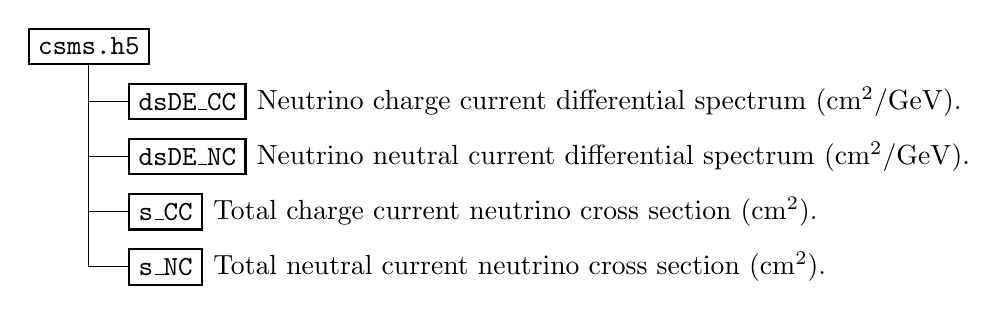
\begin{tikzpicture}[%
    grow via three points={one child at (0.5,-0.7) and
      two children at (0.5,-0.7) and (0.5,-1.4)},
    edge from parent path={(\tikzparentnode.south) |- (\tikzchildnode.west)}]
    \node {{\ttf csms.h5}}
    child { node [label=right:{Neutrino charge current differential spectrum (${\rm cm^2/GeV}$).}]  {\ttf dsDE\_CC}}
    child { node [label=right:{Neutrino neutral current differential spectrum (${\rm cm^2/GeV}$).}] {\ttf dsDE\_NC}}
    child { node [label=right:{Total charge current neutrino cross section (${\rm cm^2}$).}]{\ttf s\_CC}}
    child { node [label=right:{Total neutral current neutrino cross section (${\rm cm^2}$).}] {\ttf s\_NC}}
    ;
  \end{tikzpicture}
  \caption{HDF5 cross section format.}
  \label{fig:nusquids_cross_section_hdf5}
\end{figure}


\subsubsection{Constructors}

\begin{itemize}
\item Default constructor.
  \begin{lstlisting}
    NeutrinoDISCrossSectionsFromTables();
  \end{lstlisting}
  This constructor load the defaults {\ttf csms.h5} file
\end{itemize}

The files to load the different cross-sections can be specified
explicitly as follows. 
\begin{lstlisting}
  NeutrinoDISCrossSectionsFromTables csh5('./csms.h5');
  NeutrinoDISCrossSectionsFromTables cstxt('./nusigma_');
\end{lstlisting}

\subsubsection{Functions}

\begin{itemize}
\item Total cross sections
  \begin{lstlisting}
    double TotalCrossSection(double Enu,
    	NeutrinoFlavor flavor, NeutrinoType neutype,
    	Current current) const;
      \end{lstlisting}
      
  Returns the total cross section at an energy {\ttf Enu} in eV, neutrino
  flavor {\ttf flavor}, neutrino type: {\ttf neutype}, and {\ttf
    current} can be either {\ttf NC} or {\ttf CC} for neutral or
  charge current DIS cross sections. Using a linear interpolation in
  the logarithm of the neutrino energy. 
     
\item Single differential cross sections              
  \begin{lstlisting}
    double SingleDifferentialCrossSection(double E1, double E2,
    	NeutrinoFlavor flavor, NeutrinoType neutype,
    	Current current) const;
  \end{lstlisting}
      Function that given an incident neutrino energy ({\ttf E1}) in eV an outgoing lepton energy ({\ttf E2}), as well as neutrino flavor,
       type, and process, returns the differential cross section with
       respect to the outgoing lepton energy in ${\rm cm}^2/{\rm
         GeV}$. Using a bi-linear interpolation. 
\end{itemize}

\subsubsection{GlashowResonanceCrossSection}

This class implements the formulas in~\citep{GhandiReno} in order to calculate the electron antineutrino Glashow resonance cross section contribution.

\subsubsection{Constructors}

\begin{itemize}
\item Default constructor.
  \begin{lstlisting}
    GlashowResonanceCrossSection();
  \end{lstlisting}
\end{itemize}

\subsubsection{Functions}

\begin{itemize}
\item Total cross sections
  \begin{lstlisting}
    double TotalCrossSection(double Enu,
    	NeutrinoFlavor flavor, NeutrinoType neutype,
    	Current current) const;
  \end{lstlisting}
     Returns the total cross section in cm$^2$ at an energy {\ttf Enu} in eV, neutrino flavor {\ttf flavor}, and neutrino type: {\ttf neutype}.
     If the flavor is not electron and neutrino type is not antineutrino it returns zero.              
\item Single differential cross sections
  \begin{lstlisting}
    double SingleDifferentialCrossSection(double E1, double E2,
    	NeutrinoFlavor flavor, NeutrinoType neutype,
    	Current current) const;
  \end{lstlisting}
  Returns the single differential cross section in cm$^2$/GeV for an incident neutrinos energy ({\ttf
    E1}) in eV an outgoing neutrinos energy ({\ttf E2}) in eV, neutrino flavor ({\ttf flavor}), 
  and neutrino type ({\ttf neutype}).
     If the flavor is not electron and neutrino type is not antineutrino it returns zero.   
      
\end{itemize}

\subsection{TauDecaySpectra}

This object can be query to obtain $\tau$ decay physics into leptons
and hadrons. The formulas implemented in this class were taken
from~\citep{Dutta:2000jv}. It is only used when $\tau$-regeneration is
activated and it returns the following quantities on the energy
nodes, 
\begin{equation}
\frac{dN^{lep/had}_{dec} (E_\tau, E_\nu)}{dE_\nu} {\rm ~~and~~ }
\frac{d\bar{N}^{lep/had}_{dec} (E_\tau, E_\nu)}{dE_\nu},
\label{eqn:tau-dist}
\end{equation}
i.e. the neutrino and antineutrino spectral distributions from $\tau$
leptonic and hadronic decay modes. 

\subsubsection{Constructors and Initializing Functions}

\begin{itemize}
\item Default constructor.
  \begin{lstlisting}
    TauDecaySpectra();
  \end{lstlisting}
\item Constructor and initializing function with memory reservation.
  \begin{lstlisting}
    TauDecaySpectra(marray<double,1> E_range);
    void Init(marray<double,1> E_range);
  \end{lstlisting}
This constructor and initialization functions calculate and store the
$\tau$ decay spectra on nodes specified by the one dimensional array
{\ttf E\_range} in eV.
\end{itemize}

\subsubsection{Functions}

The following functions assume that the $\tau$ and $\bar{\tau}$ have
the same decay distribution. 

\begin{itemize}
\item (Anti)Neutrino spectra with respect to neutrino energy.
  \begin{lstlisting}
    double dNdEnu_All(int e1,int e2) const;
  \end{lstlisting}
  Returns neutrino decay spectra evaluated from energy node
  {\ttfamily e1} to energy node {\ttfamily e2} when $\tau$ decays into
  leptons or hadrons.  
  \begin{lstlisting}
    double dNdEnu_Lep(int e1,int e2) const;
  \end{lstlisting}
  Returns neutrino decay spectra evaluated between energy nodes
  {\ttfamily e1} and {\ttfamily e2} when $\tau$ decays into leptons. 
\item (Anti)Neutrino spectra with respect to $\tau$ energy.
  \begin{lstlisting}
    double dNdEle_All(int e1,int e2) const;
  \end{lstlisting}
  Returns neutrino decay spectra evaluated between energy nodes
  {\ttfamily e1} and {\ttfamily e2} when $\tau$ decays into leptons
  or hadrons with respect to the initial $\tau$ energy.
  \begin{lstlisting}
    double dNdEle_Lep(int e1,int e2) const;
  \end{lstlisting}
  Returns neutrino decay spectra evaluated between energy nodes
  {\ttfamily e1} and {\ttfamily e2} when $\tau$ decays into
  leptons with respect to the initial $\tau$ energy.
\item Get the $\tau$ branching ratio to leptons.
  \begin{lstlisting}
    double GetTauToLeptonBranchingRatio() const;
  \end{lstlisting}
  Returns the $\tau$ branching ratio to leptons.
\item Get the $\tau$ branching ratio to hadrons.
  \begin{lstlisting}
    double GetTauToHadronBranchingRatio() const;
  \end{lstlisting}
  Returns the $\tau$ branching ratio to hadrons.
\end{itemize}

\subsection{nuSQUIDS}

This object is an specialization of the {\ttf SQUIDS} class~\citep{SQUIDS} that implements the
differential equations as described in Sec.~\ref{sec:theory}. In
particular, it is used to specify the propagation {\ttf Body} and its
associated {\ttf Track}. Moreover, it uses the {\ttf
  NeutrinoCrossSections} and {\ttf TauDecaySpectra} in order to
evaluate the neutrino cross sections and $\tau$ decay spectra; the
latter is only used then {\it $\tau$} regeneration is
enabled. Furthermore, it enables the user to modify the neutrino
oscillation parameters as well as the differential equation numerical
precision. Finally, it also has the capability to create and read HDF5
files that store the program results and configuration. 

\subsubsection{Constructors}

\begin{itemize}
\item Default constructor.
  \begin{lstlisting}
    nuSQUIDS();
  \end{lstlisting}
\item Move constructor.
  \begin{lstlisting}
    nuSQUIDS(nuSQUIDS&&);
  \end{lstlisting}
Constructs a {\ttf nuSQUIDS} object from an r-value reference.  
\item Single energy mode constructor.
  \begin{lstlisting}
    nuSQUIDS(unsigned int numneu, NeutrinoType NT);
  \end{lstlisting}
This constructor and initialization function initializes {\ttfamily nuSQUIDS} in the
single energy mode. {\ttfamily numneu} specifies the number of
neutrino flavors which can go from two to six, while {\ttfamily NT} can be
set to  {\ttfamily neutrino} or {\ttfamily antineutrino}. 
\item Multiple energy mode constructor.
  \begin{lstlisting}
    nuSQUIDS(marray<double,1> E_vector,
    unsigned int numneu,NeutrinoType NT = both,
    bool iinteraction = false,
    std::shared_ptr<NeutrinoCrossSections> ncs = nullptr)
  \end{lstlisting}
This constructor and initialization function initializes {\ttfamily nuSQUIDS} in the
multiple energy mode. We need to provide the following arguments:
list of neutrino energy nodes
(\lstinline[columns=fixed,breaklines=true]{E_vector}),
number of neutrino flavors ({\ttf numneu}), neutrino or
anti-neutrino type ({\ttf NT}),  non-coherent scattering
interactions ({\ttf iinteraction}), and neutrino cross section object
pointer ({\ttf ncs}).  

\item Constructing from a $\nu$SQuIDS-HDF5 file
  \begin{lstlisting}
    nuSQUIDS(std::string hdf5_filename, std::string grp = "/",
    std::shared_ptr<InteractionStructure> int_struct = nullptr)
  \end{lstlisting}
This constructor initializes {\ttfamily nuSQUIDS} from a 
previously generated $\nu$SQuIDS HDF5 file. {\ttfamily filepath} must
specify the full path of the HDF5 file, {\ttfamily grp} specifies the
location on the HDF5 file structure where the object will be saved (by default
it will be saved on the {\ttfamily root} of the HDF5 file), and {\ttf
  int\_struct} can specify the cross-section object instead of loading it from
the file.
\end{itemize}

\subsubsection{Functions}

\textbf{Functions to evaluate flavor and mass composition}

\begin{itemize}
\item Flavor composition evaluator (single energy mode)
  \begin{lstlisting}
    double EvalFlavor(unsigned int flv) const;
  \end{lstlisting}
Returns the content a given neutrino flavor specified by {\ttfamily
  flv} ({\ttfamily 0 = $e$}, {\ttfamily 1 = $\mu$}, {\ttfamily 2 =
  $\tau$}, ...). This function can only be use in the single energy
mode. 
\item Flavor composition evaluator (multiple energy mode)
  \begin{lstlisting}
    double EvalFlavorAtNode(unsigned int flv, unsigned int ie, 
                            unsigned int rho=0) const;
    double EvalFlavor(unsigned int flv, double enu,
                      unsigned int rho=0) const;
    double EvalFlavor(unsigned int flv,double enu,
                      unsigned int rho,double scale,
                      std::vector<bool>& avr) const;
  \end{lstlisting}
{\ttfamily EvalFlavorAtNode} returns the content a given neutrino
flavor specified by {\ttfamily flv} ({\ttfamily 0 = $e$}, {\ttfamily 1
  = $\mu$}, {\ttfamily 2 = $\tau$, ...}) at an energy node {\ttfamily
  ie}. Furthermore, {\ttfamily EvalFlavor} returns the approximate
content of a given flavor for a specific neutrino energy  {\ttf enu}
by interpolating in the interaction basis. In each function, when
considering  {\ttf  NT = both}, the parameter {\ttf rho} toggles
between {\ttf neutrino (0)} and {\ttf antineutrino (1)}.
The last function gets two additional arguments: an {\ttf scale} such
that all $H_0$ induced oscillation frequencies larger than this scale
will be averaged and a vector of booleans which entries will be set to
true if the corresponding oscillations frequencies have been averaged
out.


\item Mass composition evaluator (single energy mode)
  \begin{lstlisting}
    double EvalMass(unsigned int eig) const;
  \end{lstlisting}
Returns the content a given neutrino mass eigenstate specified by {\ttfamily eig} ({\ttfamily 0 = $\nu_1$}, {\ttfamily 1 = $\nu_2$}, {\ttfamily 2 = $\nu_3$, ...}). This function can only be use in the  single energy mode.
\item Mass composition evaluator (multiple energy mode)
  \begin{lstlisting}
    double EvalMassAtNode(unsigned int eig, unsigned int ie,
                           unsigned int rho=0) const;
    double EvalMass(unsigned int eig, double enu,
                     unsigned int rho=0) const;
    double EvalMass(unsigned int flv,double enu,
                    unsigned int rho,double scale,
                    std::vector<bool>& avr) const;
  \end{lstlisting}
{\ttfamily EvalMassAtNode} returns the content a given neutrino mass
eigenstate specified by {\ttfamily eig} ({\ttfamily 0 = $\nu_1$},
{\ttfamily 1 = $\nu_2$}, {\ttfamily 2 = $\nu_3$, ...}) at an energy
node {\ttfamily ie}. Furthermore, {\ttfamily EvalMass} returns the
approximate content of a given mass eigenstate for a specific neutrino
energy  {\ttf enu} by interpolating in the interaction basis. In each
function, when considering  {\ttf  NT = both}, the parameter {\ttf
  rho} toggles between {\ttf neutrino (0)} and {\ttf antineutrino
  (1)}. The last function gets two additional arguments: an {\ttf scale} such
that all $H_0$ induced oscillation frequencies larger than this scale
will be averaged and a vector of booleans which entries will be set to
true if the corresponding oscillations frequencies have been averaged
out.
\end{itemize}

\textbf{Functions to evolve the neutrino ensemble}

\begin{itemize}
\item Evolve state
  \begin{lstlisting}
    void EvolveState();
  \end{lstlisting}
Once the neutrino propagation problem has been setup this function
evolves the neutrino state from its initial position to its final
position specified by the {\ttfamily track}. 
\end{itemize}

\textbf{Functions obtain properties of the nuSQUIDS object as well as the state}

\begin{itemize}
\item Get energy nodes values
  \begin{lstlisting}
    marray<double,1> GetERange() const;
  \end{lstlisting}
  Returns a one dimensional array containing the energy nodes
  positions given in eV. 
  \item Get number of energy nodes
  \begin{lstlisting}
    unsigned int GetNumE() const;
  \end{lstlisting}
  Returns the number of energy nodes.
  \item Get number neutrino flavors
  \begin{lstlisting}
    unsigned int GetNumNeu() const;
  \end{lstlisting}
  Returns the number of neutrino flavors.
  \item Get Hamiltonian at current position
  \begin{lstlisting}
    SU_vector GetHamiltonian(unsigned int ie, 
                             unsigned int rho = 0);
  \end{lstlisting}
  Returns the {\ttf SU\_vector} that represents the (anti)neutrino
  Hamiltonian at the current position, at a given energy node {\ttf
    ie}, and  {\ttf rho} specifies whether the neutrino or antineutrino.
  \item Get the state of the system 
  \begin{lstlisting}
      const squids::SU_vector& GetState(unsigned int ei,unsigned int rho = 0) const;
  \end{lstlisting}
  Returns the {\ttf SU\_vector} that represents the (anti)neutrino state at given energy node {\ttf ie}. 
  Furthermore, {\tt rho} specifies whether the neutrino or antineutrino state is returned.
  \item Get the flavor projector
  \begin{lstlisting}
    SU_vector GetFlavorProj(unsigned int ie, unsigned int rho = 0) const;
  \end{lstlisting}
  Returns a {\ttf SU\_vector} that represents the flavor projector for the energy node {\ttf ie} and 
  {\ttf rho} specifies if neutrinos or antineutrinos are requested.
  \item Get the mass projector
  \begin{lstlisting}
    SU_vector GetMassProj(unsigned int ie, unsigned int rho = 0) const;
  \end{lstlisting}
  Returns a {\ttf SU\_vector} that represents the mass projector for the energy node {\ttf ie} and 
  {\ttf rho} specifies if neutrinos or antineutrinos are requested.
  \item Get {\ttfamily Body}
  \begin{lstlisting}
    std::shared_ptr<Body> GetBody() const;
  \end{lstlisting}
  Returns the {\ttf Body} instance currently stored in the {\ttf nuSQUIDS} object.
  \item Get {\ttfamily Track}
  \begin{lstlisting}
    std::shared_ptr<Track> GetTrack() const;
  \end{lstlisting}
  Returns the {\ttf Track} instance currently stored in the {\ttf nuSQUIDS} object.
  \item Get mixing angle
  \begin{lstlisting}
    double Get_MixingAngle(unsigned int i, unsigned int j) const;
  \end{lstlisting}
  Returns the $\theta_{i,j}$ mixing angle where {\ttf i} and {\ttf j} are zero based indexes.
  \item Get CP phase
  \begin{lstlisting}
    double Get_CPPhase(unsigned int i, unsigned int j) const;
  \end{lstlisting}
  Returns the $\delta_{i,j}$ CP phase where {\ttf i} and {\ttf j} are zero based indexes.
  \item Get square mass difference
  \begin{lstlisting}
    double Get_SquareMassDifference(unsigned int i) const;
  \end{lstlisting}
  Returns the $\Delta m^2_{i0}$ in ${\rm eV}^2$ where $1\le i < {\rm \tt numneu}$.
  \end{itemize}
  
\textbf{Functions to set properties of the nuSQUIDS object as well as the state}

\begin{itemize}
  \item Set {\ttfamily Body}
  \begin{lstlisting}
    void Set_Body(std::shared_ptr<Body>);
  \end{lstlisting}
  Sets the {\ttf Body} instance in which the neutrino propagation will take place.
  \item Set {\ttfamily Track}
  \begin{lstlisting}
    void Set_Track(std::shared_ptr<Track>);
  \end{lstlisting}
  Sets the {\ttf Track} instance which describes the neutrino propagation inside a
  given {\ttf Body}.
  \item Set the initial state
  \begin{lstlisting}
    void Set_initial_state(marray<double,1> state, Basis basis);
    void Set_initial_state(marray<double,2> state, Basis basis);
    void Set_initial_state(marray<double,3> state, Basis basis);
  \end{lstlisting}
  {\ttf Set\_initial\_state} sets the initial neutrino (and
  antineutrino) state. The states  can be specified for the single and
  multiple energy modes can be specified using the different {\ttf
    C++} signatures. In each case {\ttf basis} can be either {\ttf
    mass} or {\ttf flavor}. 
  \begin{itemize}
  	\item {\ttf marray<double,1> state}: 
	Can only be used in single energy mode and is defined by 
	{\ttf state[$\alpha$]  = $\phi_\alpha$ } where $\alpha$ is a
        flavor or mass eigenstate index. 
	\item {\ttf marray<double,2> state}: Can only be used in
          multiple energy mode and is defined by {\ttf
            state[ei][$\alpha$]  = $\phi_\alpha (E$[ei]$),$ } i.e. the
          flavor (mass) eigenstate composition at a given energy node
          {\ttf ei}. 
	\item {\ttf marray<double,3> state}: Can only be used in
          multiple energy mode and is defined by {\ttf
            state[ei][$\rho$][$\alpha$]  = $\phi^{\rho}_\alpha
            (E$[ei]$),$ } i.e. the flavor (mass) eigenstate
          composition at a given energy node {\ttf ei}, and where
          $\rho = 0 \equiv {\rm neutrino}$ and $\rho = 0 \equiv {\rm
            antineutrino}$. 
  \end{itemize}
  \item Set energy
  \begin{lstlisting}
    void Set_E(double enu);
  \end{lstlisting}
  Set the neutrino energy. This function can only be used in the
  single energy mode and {\ttf enu} has to be in natural units.
  \item Enable progress bar
  \begin{lstlisting}
    void Set_ProgressBar(bool opt);
  \end{lstlisting}
  If {\ttf opt} is {\ttf true} a progress bar will be printed to
  indicate the calculation progress. 
  \item Enable tau regeneration
  \begin{lstlisting}
    void Set_TauRegeneration(bool opt);
  \end{lstlisting}
  If {\ttf opt} is {\ttf true}, {\ttf NT} is {\ttf both}, and non
  coherent interactions are enabled tau regeneration effects will be included.
  \item Set mixing angle
  \begin{lstlisting}
    void Set_MixingAngle(unsigned int i, unsigned int j, double angle);
  \end{lstlisting}
  Sets the $\theta_{i,j}$ mixing angle to {\ttf angle}, where {\ttf i}
  and {\ttf j} are zero based indexes, and {\ttf angle} must be given in radians.
  \item Get CP phase
  \begin{lstlisting}
    void Set_CPPhase(unsigned int i, unsigned int j, doble phase);
  \end{lstlisting}
  Sets the $\delta_{i,j}$ CP phase to {\ttf phase}, where {\ttf i} and
  {\ttf j} are zero based indexes, and {\ttf phase} must be given in radians.
  \item Set square mass difference
  \begin{lstlisting}
    void Set_SquareMassDifference(unsigned int i, doble dmsq);
  \end{lstlisting}
  Sets the $\Delta m^2_{i0}$ to {\ttf dams}, given in ${\rm eV}^2$,
  where $1\le i < {\rm \tt numneu}$. 
  \item Set parameters to default
  \begin{lstlisting}
    void Set_MixingParametersToDefault();
  \end{lstlisting}
  Sets the mixing angles and square mass mixings to the best fit point
  given in \citep{Gonzalez-Garcia:2014bfa}. 
  \item Set the basis of solution
  \begin{lstlisting}
    void Set_Basis(Basis basis);
  \end{lstlisting}
  Sets the basis on which the evolution will be performed. Two options
  are available: {\ttf mass} and {\ttf interaction}, the later being
  the default. 
\item Set neutrino cross-section
  \begin{lstlisting}
    void SetNeutrinoCrossSections(std::shared_ptr<NeutrinoCrossSections> xs)
  \end{lstlisting}
  Sets the neutrino cross-section~\ref{sec:xs} given by the shared
  pointer {\ttf xs} to the nuSQuIDS object.
\end{itemize}
  
\textbf{HDF5 interface functions}
 
\begin{itemize}
  \item Write nuSQUIDS object into an HDF5 file.
  \begin{lstlisting}
    void WriteStateHDF5(std::string hdf5_filename,
                        std::string group = "/",
                        bool save_cross_sections = true, 
                        std::string cross_section_grp_loc = "") const;
  \end{lstlisting}
  Writes the current {\ttf nuSQUIDS} configuration and state into an HDF5 file
  for later use. {\ttf hdf5\_filename} specifies the output filename, {\ttf group} is the 
  location on the HDF5 structure where the {\ttf nuSQUIDS} object will be save; by default
  the root of the HDF5 will be used. Furthermore, {\ttf
    save\_cross\_sections} and {\ttf cross\_section\_grp\_loc} specify
  if cross sections will be saved and where on the HDF5 file
  structure. See Figure~\ref{fig:nusquids_hdf5}. 
  \item Add to the HDF5 write funtion.
  \begin{lstlisting}
    virtual void AddToWriteStateHDF5(hid_t hdf5_loc_id) const;
  \end{lstlisting}
  En ables the user to add content in the HDF5 file. An HDF5
  location,{\ttf hdf5\_loc\_id}. Using that the user can stor relevant
  informa about the derived nuSQuIDS class.
  \item Read nuSQUIDS object from an HDF5 file.
    \begin{lstlisting}
    void ReadStateHDF5(std::string hdf5_filename,
                       std::string group = "/",
                       std::string cross_section_grp_loc = "");
  \end{lstlisting}
  Reads an previously generated HDF5 file and sets the {\ttf nuSQUIDS} object
  accordingly, i.e. it configures it and loads the saved state. {\ttf
    hdf5\_filename} specifies the input filename, {\ttf group} is the
  location on the HDF5 structure where the {\ttf nuSQUIDS} object is;
  by default the root of the HDF5 is assumed. Furthermore, {\ttf
    cross\_section\_grp\_loc} specify where the cross sections are in
  the HDF5 file structure. See Figure~\ref{fig:nusquids_hdf5}. 
  \item Add to the HDF5 read file.
  \begin{lstlisting}
    virtual void AddToReadStateHDF5(hid_t hdf5_loc_id);
  \end{lstlisting}
  Enables the user to read user defined content from the HDF5 file. An
  HDF5 location,{\ttf hdf5\_loc\_id}, is provided so the user can
  interface with the HDF5 library. For a correct implementations this
  functions has to be implemented consistently with {\ttf
    AddToWriteStateHDF5} function. 
\end{itemize}

\begin{figure}[htb]
\centering
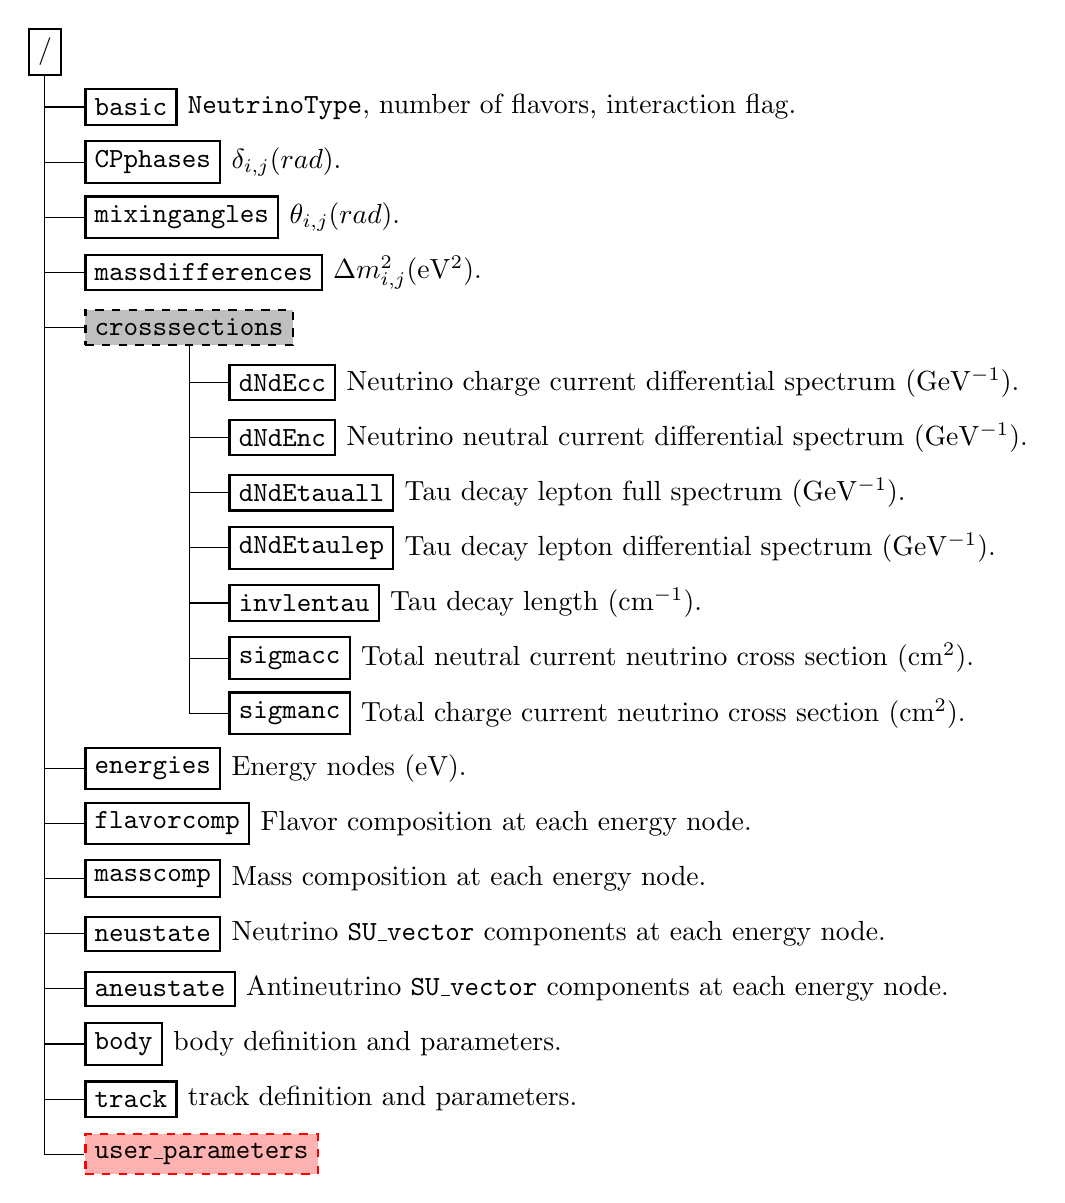
\begin{tikzpicture}[%
  grow via three points={one child at (0.5,-0.7) and
  two children at (0.5,-0.7) and (0.5,-1.4)},
  edge from parent path={(\tikzparentnode.south) |- (\tikzchildnode.west)}]
  \node {/}
    child { node [label=right:{{\ttf NeutrinoType}, number of flavors, interaction flag.}] {\ttf basic}}	
    child { node [label=right:{$\delta_{i,j} (rad).$}] {\ttf CPphases}}		
    child { node [label=right:{$\theta_{i,j} (rad).$}] {\ttf mixingangles}}
    child { node [label=right:{$\Delta m^2_{i,j} (\rm eV^2).$}] {\ttf massdifferences}}
    child { node [optional] {\ttf crosssections}
      child { node [label=right:{Neutrino charge current differential spectrum (${\rm GeV^{-1}}$).}]  {\ttf dNdEcc}}
      child { node [label=right:{Neutrino neutral current differential spectrum (${\rm GeV^{-1}}$).}] {\ttf dNdEnc}}
      child { node [label=right:{Tau decay lepton full spectrum (${\rm GeV^{-1}}$).}] {\ttf dNdEtauall}}
      child { node [label=right:{Tau decay lepton differential spectrum (${\rm GeV^{-1}}$).}] {\ttf dNdEtaulep}}
      child { node [label=right:{Tau decay length (${\rm cm^{-1}}$).}] {\ttf invlentau}}
      child { node [label=right:{Total neutral current neutrino cross section (${\rm cm^2}$).}]{\ttf sigmacc}}
      child { node [label=right:{Total charge current neutrino cross section (${\rm cm^2}$).}] {\ttf sigmanc}}
    }
    child [missing] {}				
    child [missing] {}				
    child [missing] {}
    child [missing] {}
    child [missing] {}			
    child [missing] {}
    child [missing] {}			
    child { node [label=right:{Energy nodes ({\rm eV}).}] {\ttf energies}}	
    child { node [label=right:{Flavor composition at each energy node.}] {\ttf flavorcomp}}
    child { node [label=right:{Mass composition at each energy node.}] {\ttf masscomp}}
    child { node [label=right:{Neutrino {\ttf SU\_vector} components at each energy node.}] {\ttf neustate}}
    child { node [label=right:{Antineutrino {\ttf SU\_vector} components at each energy node.}] {\ttf aneustate}}
    child { node [label=right:{body definition and parameters.}] {\ttf body}}
    child { node [label=right:{track definition and parameters.}] {\ttf track}}
    child { node [selected] {\ttf user\_parameters}}
    ;
\end{tikzpicture}
\caption{Structure of {\ttf nuSQUIDS} HDF5 file. The {\ttf
    crosssections} group will only be written when interactions are
  enable. Furthermore, {\ttf user\_parameters} are by default empty
  and can be set/access by {\ttf AddToWriteStateHDF5/AddToReadStateHDF5}.} 
\label{fig:nusquids_hdf5}
\end{figure}


\newcommand{\jt}[2]{
\item[$\circ$]{#1}
  \begin{lstlisting}
    {#2}
  \end{lstlisting}
}

\subsection{nuSQUIDSAtm}

Atmospheric neutrino oscillations is a major and instrumental part of
research in contemporary neutrino physics. Experiments like
SuperKamiokande, IceCube, and Antares have used atmospheric neutrinos
to measure neutrino mass splittings and mixing angles. Furthermore,
proposed extensions like HyperKamiokande, PINGU, and ORCA ought to
improve the current measurements and have sensitivity to neutrino
neutrino mass ordering. This class allows to propagate a set of full
energy spectrum of neutrinos for a different number of zenith angles.
It implements functions to set easily the initial conditions and also
interpolations to get the fluxes.
\subsubsection{Constructors}

\begin{itemize}
\item[$\circ$] Constructor with {\ttf costh} range.
  \begin{lstlisting}
    template<typename... ArgTypes> nuSQUIDSAtm(double costh_min, 
                                               double costh_max,
                                               unsigned int costh_div, 
                                               ArgTypes&&... args)
  \end{lstlisting}
This constructor it creates a set {\ttf nuSQUIDS} or derived {\ttf
  nuSQUIDS} objects with a set of
{\ttf costh\_div} zenith angles from {\ttf costh\_min} to {\ttf
  costh\_max}, the last arguments are the argmunets of the base {\ttf
  nuSQUIDS} object.

\item[$\circ$] Constructor with {\ttf costh} array.
  \begin{lstlisting}
    template<typename... ArgTypes> nuSQUIDSAtm(marray<double,1> costh_array,
                                               ArgTypes&&... args):
  \end{lstlisting}
Similar to the last constructor but instead of define the boundaries
and the number of divisions the user should give as an argument an
array with the number of the zenith cosine.
\item[$\circ$] Constructing from a $\nu$SQuIDSAtm-HDF5 file
  \begin{lstlisting}
    nuSQUIDSAtm(std::string hdf5_filename);
  \end{lstlisting}
This constructor initializes {\ttfamily nuSQUIDS} from a 
previously generated $\nu$SQuIDS-HDF5 file. The result {\ttfamily nuSQUIDS} 
object will be given in {\it single} or {\it multiple} energy mode
depending on the HDF5 file configuration. {\ttfamily filepath} must specify the full
path of the HDF5 file. Furthermore,
{\ttfamily grp} specifies the location on the HDF5 file structure
where the object will be saved; by default
it will be saved on the {\ttfamily root} of the HDF5 file.
\item[$\circ$] Constructing from a $\nu$SQuIDS-HDF5 object
  \begin{lstlisting}
    nuSQUIDSAtm(nuSQUIDSAtm&&);
  \end{lstlisting}
Construct a {\ttfamily nuSQUIDSAtm} object from an existing {\ttfamily
  nuSQUIDSAtm} object through the {\ttfamily move} operator.

\end{itemize}


\subsubsection{Functions}


% TODO: section describing space and time complexity, benchmarks

\section{Python Interface}

As the particle physics community has transition from {\ttfamily FORTRAN} to {\ttfamily C++} based Monte Carlos, it is also a current trent to be able to interface particle physics software with high level interpreted languages such as {\ttfamily Mathematica}, {\ttfamily R}, and {\ttfamily Python}. Of these languages we have decided to implement bindings with Python due to the well developed {\ttfamily C++}-{\ttfamily Python} bindings given by the {\ttfamily Boost} library. In later version of this software we may incorporate interfaces to other high level languages; though, note, that in particular {\ttfamily Mathematica} architecture is not object oriented and bindings to other languages only exist in {\ttfamily C} and {\ttfamily FORTRAN}.

\subsection{Installation}

In order to install nuSQuIDS python bindings additional libraries are required, namely, {\ttfamily Boost.Python} ($\ge1.54$) and {\ttfamily Python.numpy} ($\ge1.7$). Upon installing these new prerequisites you can run the following commands to install the bindings

% TODO: this won't actually build or install the bindings
% We don't even have an install target for the bindings; we might need/want to add one

\begin{lstlisting}[language=Bash]
./config --with-python-bindings
make && make install
\end{lstlisting}

After successful installation you can import the python bindings in the following manner

\begin{lstlisting}[language=Python]
import nuSQUIDSpy as nsq
\end{lstlisting}
where here we have introduce the alias {\ttfamily nsq} for the nuSQuIDS python module. We can further extend the
capabilities of nuSQuIDS in {\ttfamily Python} by means of the the {\ttfamily nuSQUIDSTools} python module. When 
this module is loaded the nuSQuIDS functions and objects get overloaded with python only functionalities. In order to enable this, after loading the {\ttfamily nuSQUIDSpy} module, do

\begin{lstlisting}[language=Python]
import nuSQUIDSTools
\end{lstlisting}


\subsection{Description of the interface}



\subsection{Examples}

\section{Conclusions \& Acknowledgements} 
\label{sec:conclu} 

\bibliographystyle{plain}
%\bibliographystyle{elsarticle-harv}
\bibliography{nusquids}

\end{document}

